\documentclass{mcmthesis}

\mcmsetup{tstyle=\color{red}\bfseries,%修改题号，队号的颜色和加粗显示，黑色可以修改为 black
        tcn = 2503118, problem = D, %修改队号，参赛题号
        sheet = true, titleinsheet = true, keywordsinsheet = true,
        titlepage = false, abstract = true}

  %四款字体可以选择
  %\usepackage{times}
  %\usepackage{newtxtext}
  %\usepackage{palatino}
\usepackage{txfonts}

\usepackage{diagbox}
\usepackage{booktabs}
\usepackage{indentfirst}  %首行缩进，注释掉，首行就不再缩进。
\usepackage{lipsum}
\usepackage{tocloft}
\usepackage{footnote}
\setcounter{tocdepth}{2}
\usepackage[numbers,super]{natbib}



\title{Bridge-Linked Revitalization: Resilience and Multimodal Optimization in Baltimore's Transportation System}

% \author{\small \href{https://www.latexstudio.net/}
%   {\includegraphics[width=7cm]{mcmthesis-logo}}}
% \date{\today}
\begin{document}

% 摘要页
\pagenumbering{arabic} % 使用阿拉伯数字计数页码
\setcounter{page}{1}   % 设置页面从1开始
\thispagestyle{empty}  % 隐藏摘要页的页码

\begin{abstract}
  
 \par
  

Our study addresses the vulnerability of \textbf{urban transportation networks} and the conflicting needs of \textbf{multiple stakeholders} following the \textbf{Francis Scott Key Bridge} collapse in Baltimore. Using \textbf{Voronoi diagram partitioning} and \textbf{topological network modeling}, combined with AADT traffic data and \textbf{stakeholder preference analysis}, we quantify the multidimensional impacts of the collapse on \textbf{traffic flow}, \textbf{economic activity}, and \textbf{community resilience}. Findings show that the collapse reduced peak-hour speeds on I-95 and I-895 to 10 mph, increased freight costs by 18\%, and extended commuter travel times by 41\%, highlighting the risks of single-point-dependent transportation networks.

We propose a \textbf{resilience-driven optimization framework} with three core strategies. First, recalibrating 82 signalized intersections and constructing \textbf{three port connectors} improve I-95 throughput by \textbf{25\%} and reduce EMS response times to 8 minutes, alleviating congestion and enhancing \textbf{network resilience}. Second, a \$73 million investment in 5 km of protected bike lanes and pedestrian pathways is projected to reduce commute times by 15\%, cut CO₂ emissions by \textbf{10\%}, and enhance disaster evacuation capacity in 56\% of low-vegetation areas, promoting \textbf{sustainable urban development}. Third, integrating \textbf{intelligent transportation systems} enables real-time monitorin and \textbf{dynamic signal optimization}, improving network efficiency and equity.

The study identifies implementation challenges, including a 28\% local funding gap and land-use coordination complexities. We recommend prioritizing \textbf{non-motorized projects} and phasing \textbf{arterial upgrades}, supported by \textbf{interagency coordination} and \textbf{real-time traffic monitoring platforms}. Spatial analysis using \textbf{Voronoi tessellation} reveals significant disparities in \textbf{transportation service quality}, with the southern region’s accessibility index at 0.44 compared to the central region’s 2.13, indicating urgent improvements are needed.

This research advances \textbf{urban resilience planning} by developing a \textbf{replicable methodology} that integrates \textbf{geospatial analysis} with \textbf{stakeholder-centric modeling}. It demonstrates how infrastructure redundancy and intelligent systems can enhance \textbf{operational efficiency} and \textbf{social equity}, providing a \textbf{scientific foundation} for Baltimore’s recovery plan and establishing a \textbf{new paradigm} for \textbf{equitable transportation planning} in port cities facing similar challenges.


\begin{keywords}
Urban Transportation Networks; Voronoi Diagram Partitioning; Resilience-driven Optimization Framework; Stakeholder Preference Analysis; Freight Cost Increase; Commuter Travel Times; Intelligent Transportation Systems; Equitable Transportation Planning; Sustainable Urban Development
\end{keywords}


\end{abstract}


\maketitle
%% Generate the Table of Contents, if it's needed.
% 目录页
\newpage
\thispagestyle{empty}  % 隐藏目录页的页码
\tableofcontents



\newpage
\pagenumbering{arabic} % 正常的页码显示方式
\setcounter{page}{3}   % 如果想要正文从某个页码开始，设置初始页码

%1
\section{Introduction}
%1.1
\subsection{Problem Background}

As a critical hub in urban transportation networks, cross-sea bridges hold irreplaceable strategic value in regional connectivity, economic synergy, and social services. Baltimore, a major U.S. port city, has long faced challenges from aging infrastructure, complex geography, and conflicting stakeholder demands. The collapse of the Francis Scott Key Bridge in March 2024—after being struck by a disabled container ship—severed the Chesapeake Bay's sole cross-sea transportation link, exacerbating systemic vulnerabilities. With a daily traffic volume exceeding 30,000 vehicles and handling 80\% of the bay's cross-sea freight, its absence triggered cascading effects:
\vspace{-2.9mm}
\begin{itemize}
    \item \textbf{Efficiency Loss:}Detour routes added 4 miles, increasing commute times by 15–20 minutes. Port closure rerouted 21,000 TEUs, raising logistics costs by 18\%.

    \item \textbf{Economic Impact:} The port ecosystem employed 15,000 workers and supported 140,000 indirect jobs. Post-collapse, Maryland lost \$28 million in monthly tax revenue.

    \item \textbf{Cultural Loss:}The collapse of this landmark structure—attracting 500,000 annual visitors—eroded Baltimore's cultural identity and tourism appeal.

\end{itemize}
\vspace{-2.9mm}
This event exposed vulnerabilities in single-node transportation systems while providing a case study for infrastructure redundancy, multimodal network optimization, and community equity.

\begin{figure}[ht]
    \centering
    \begin{minipage}{0.49\textwidth}
        \centering
        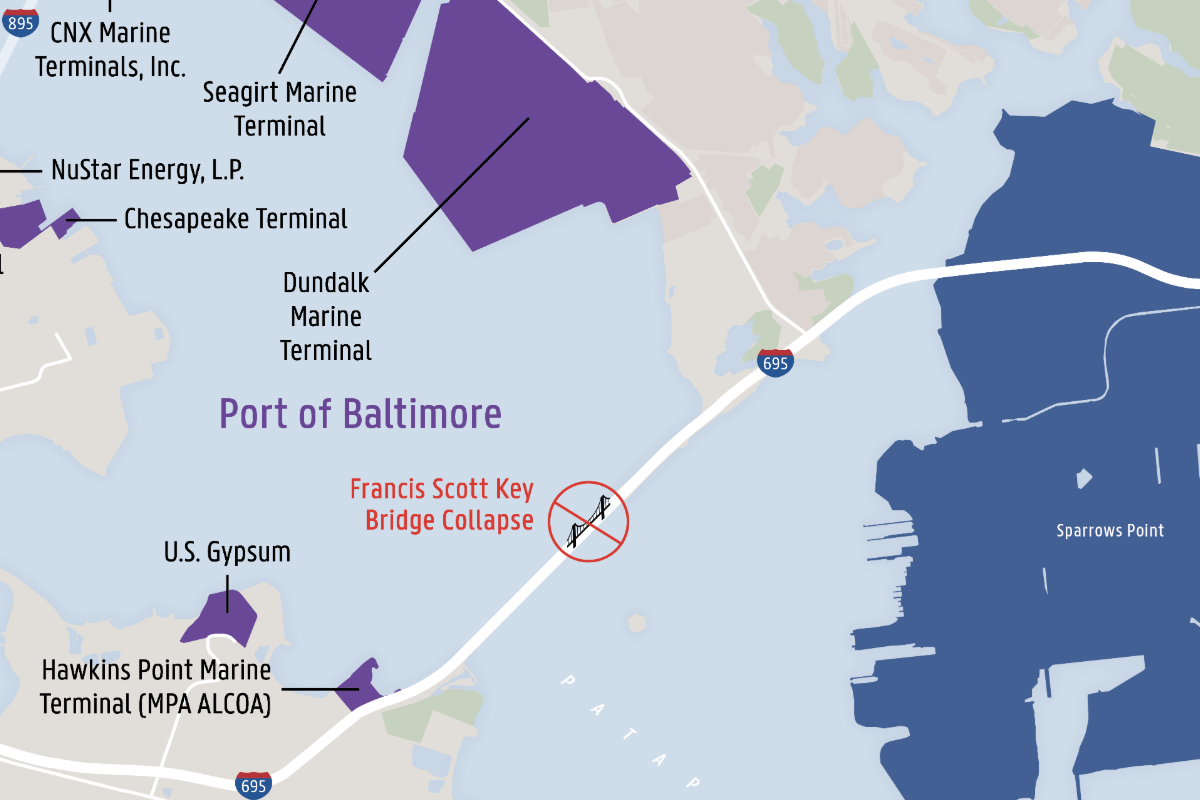
\includegraphics[width=\linewidth]{figures/Francis Scott Key Bridge地图位置.png}
        \caption{ Francis Scott Key Bridge}
        \label{fig:image1}
    \end{minipage}
    \hfill
    \begin{minipage}{0.46\textwidth}
        \centering
        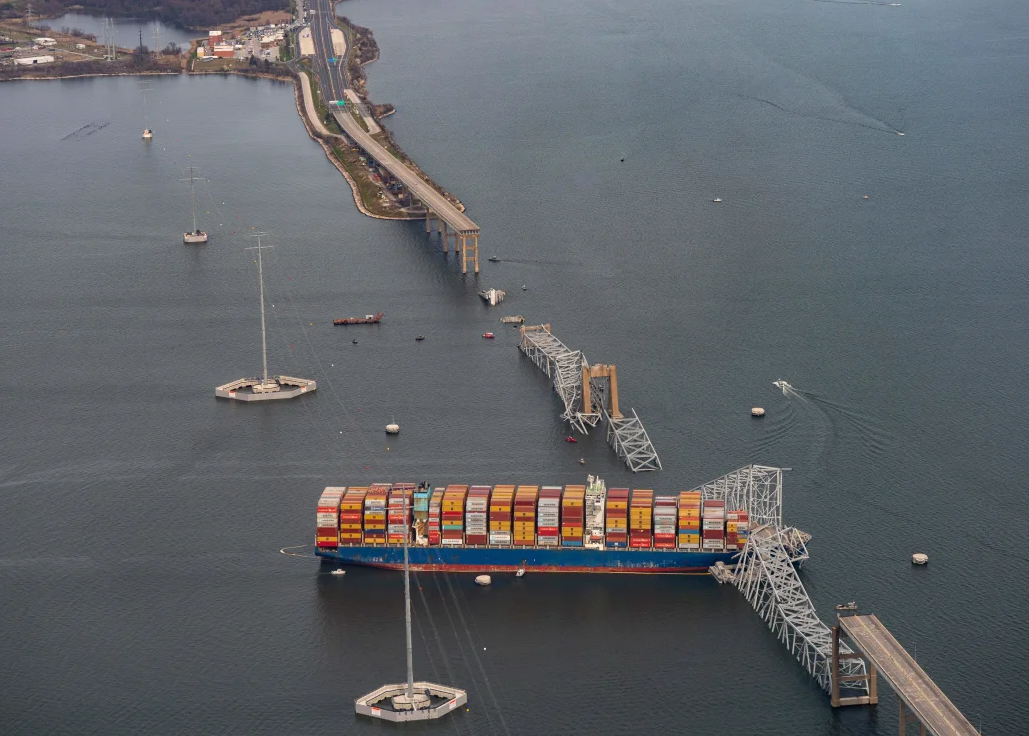
\includegraphics[width=\linewidth]{figures/bridgeCollapse.png}
        \caption{Bridge Collapse Site}
        \label{fig:image2}
    \end{minipage}
\end{figure}


\subsection{Concept Elaboration}

\textbf{(1) Infrastructure Redundancy}

Refers to backup capacity for critical nodes in transportation networks\cite{farahani2013review}. The bridge collapse highlighted the risks of single-point dependency in cross-bay connectivity. Redundancy can be enhanced through parallel bridges or multimodal alternatives (e.g., ferries, rail).

\textbf{(2) Multimodal Transportation Network Optimization}

Aims to coordinate road, public transit, and pedestrian systems to reduce conflicts and improve efficiency. Baltimore must balance highway accessibility with community connectivity, avoiding historical pitfalls like the US-40 "Highway to Nowhere" that divided neighborhoods.



\subsection{Restatement of The Tasks}

According to the data and modeling requirements of Baltimore's transportation system, we address the following problems:
\vspace{-2.9mm}
\begin{itemize}
    \item Develop real-time impact assessment network models for bridge collapses with multidimensional visualization (traffic flow/commute/logistics)

    \item Validate correlations between critical node vulnerability and catastrophic infrastructure failures in transportation networks\cite{ji2012spatial}

    \item Predict critical transition thresholds during reconstruction and identify dominant factors to formulate redundancy-driven optimization frameworks

    \item Evaluate model accuracy and generalizability to refine urban transportation planning methodologies
\end{itemize}
\vspace{-2.9mm}



\subsection{Overview of Our Works}

\begin{figure}[htbp]
    \centering
    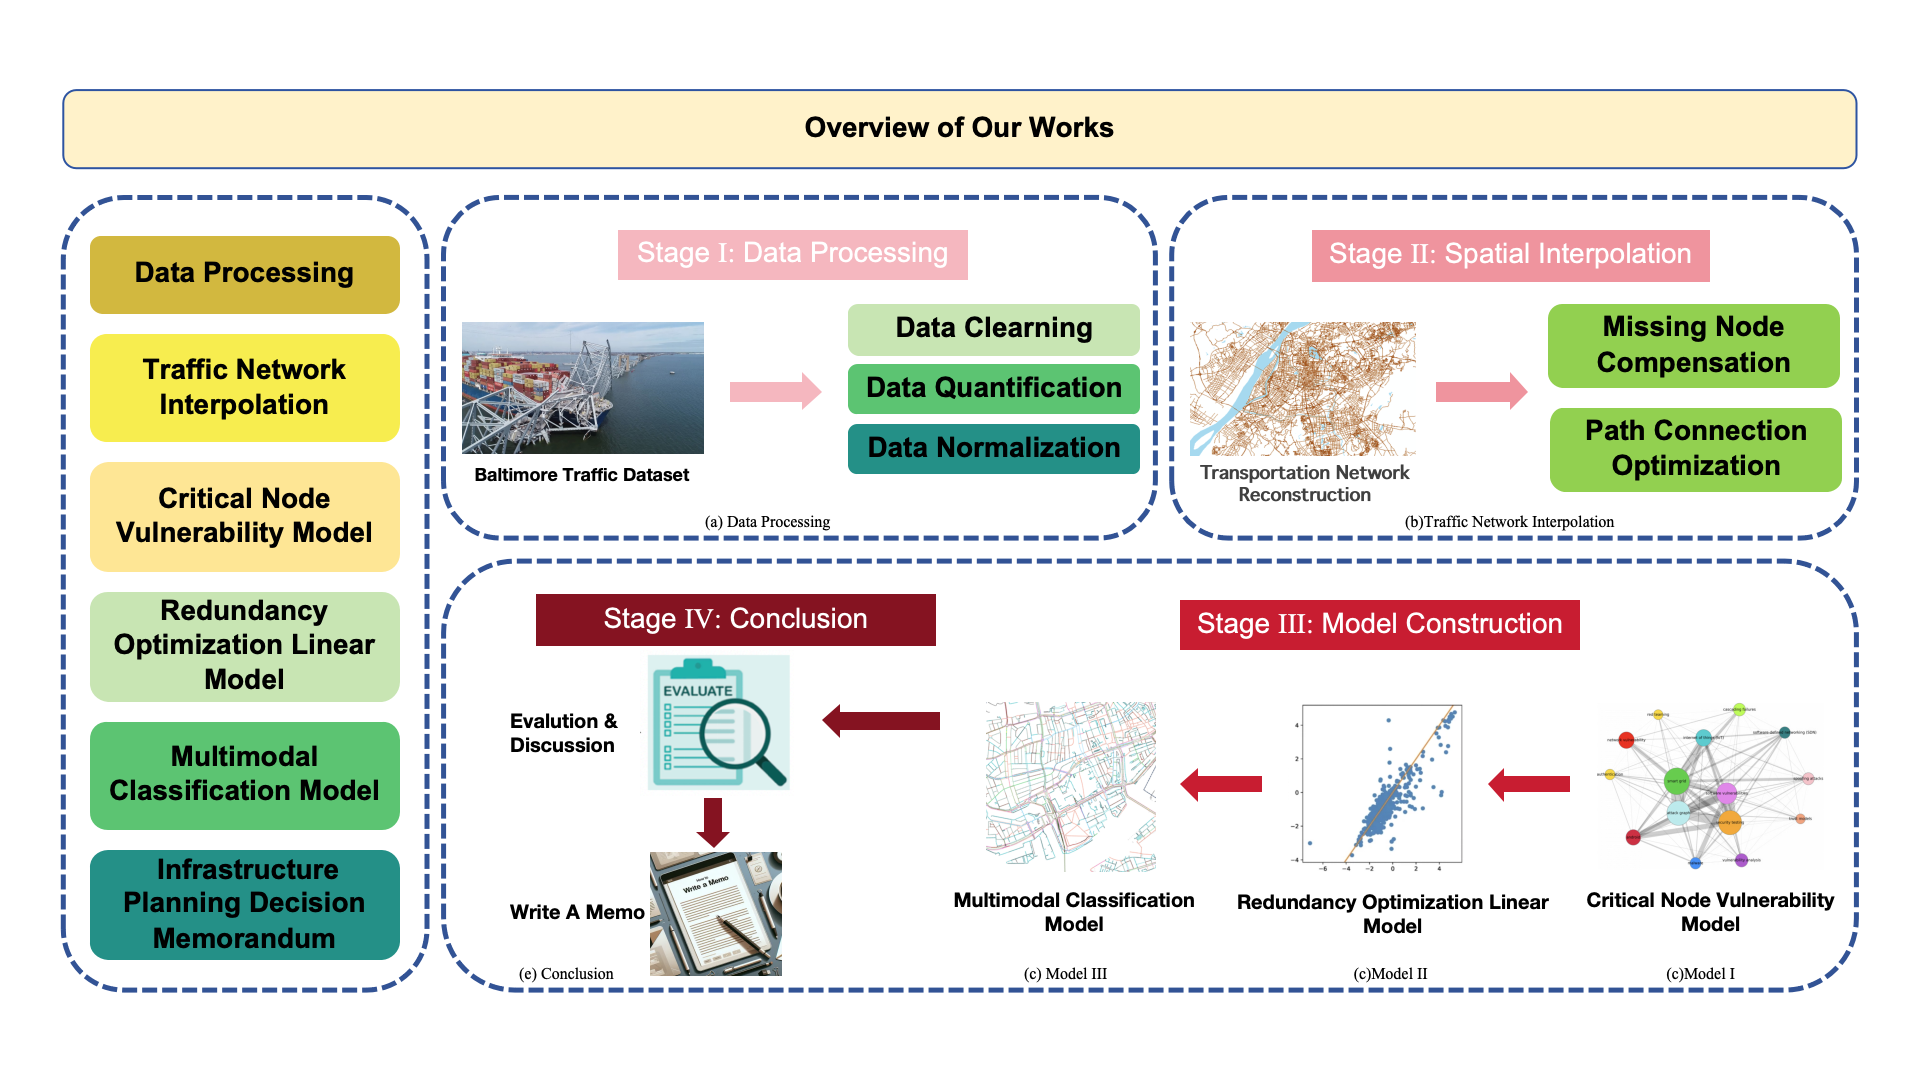
\includegraphics[width=1\linewidth]{ourWork.png}
    \caption{Our Works}
    \label{fig:enter-label}
\end{figure}






\section{General Assumptions}

\begin{itemize}
    \item \textbf{Long-term Traffic Flow Stability:}
           Historical data (2014--present
) exhibit reliability in accurately mapping real-world conditions (AADT/AAWDT).

    \item \textbf{Road Network Topology Consistency:}
          Bridge collapse alters traffic distribution/route selection without inducing structural reconfiguration.

    \item \textbf{Quantifiable Travel Demand:}
           Multi-agent mobility preferences parameterized via established behavioral models.

    \item \textbf{Traffic Control Simplification:}
          Focus on bridge failure's direct network flow impacts, marginalizing signal control variables.    
          
\end{itemize}







\section{Road Network Esrablishment}

\subsection{Basic Road Network Construction}

The construction of a basic road network from CSV data starts with data preparation and cleaning to ensure consistency and integrity, including addressing missing values. After cleaning, the data is imported into appropriate formats using Python's CSV module and converted into DataFrame structures. The arcpy and networkX libraries are then used to build and analyze the network graph, adding nodes for origins and destinations and creating edges with attributes like speed limits. Network analysis, including connectivity checks, follows graph construction.

\vspace{-2mm}
\begin{figure}[htbp]
    \centering
    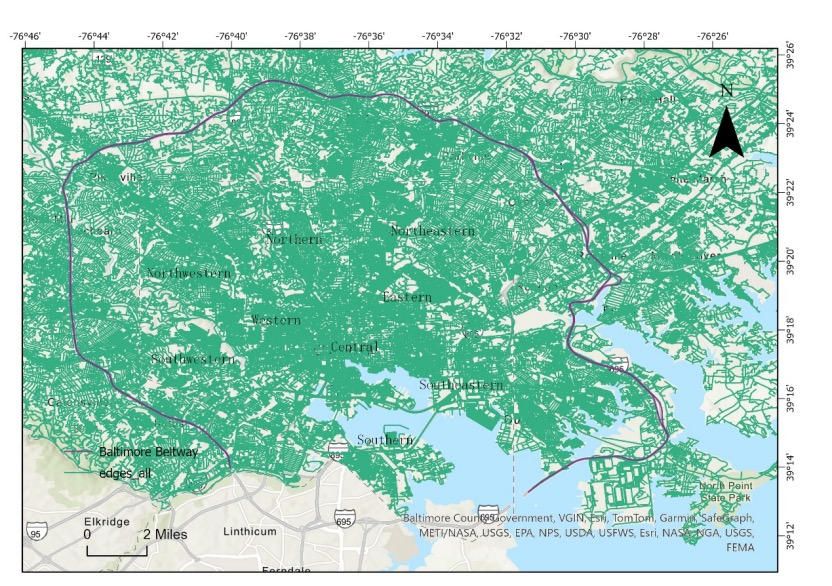
\includegraphics[width=0.75\linewidth]{figures/Urban transportation road network construction..jpg}
    \caption{Urban transportation road network construction}
    \label{fig:enter-label}
\end{figure}


\subsection{Basic Road Network Analysis}

Further analysis of the road network focuses on the highway attribute, categorizing stakeholder-specific requirements while filtering out disused road types. Different stakeholders prioritize distinct transportation needs:
\vspace{-2.9mm}
\begin{itemize}
    \item \textbf{Urban residents} prioritize the convenience of daily commuting, requiring pedestrian pathways, cycling lanes, public transit facilities, and residential streets.

    \item \textbf{Business owners} emphasize the efficiency of freight transportation and accessibility to commercial areas, requiring primary and secondary roads as well as service routes.

    \item \textbf{Suburban residents} rely on highways and arterial roads for commuting, and they also require residential streets and local access roads.

    \item \textbf{Commuter populations} require time-sensitive mobility solutions via grade-separated arterials and high-frequency transit hubs.

    \item \textbf{Transit travelers} depend on uninterrupted through-route functionality with minimized conflict points across jurisdictional boundaries.

    \item \textbf{Tourists} demand seamless multimodal connectivity to heritage sites, prioritizing pedestrian pathways, bike-sharing systems, and tourist-oriented transit services.
\end{itemize}
\vspace{-2.9mm}





Based on the prioritized requirements of diverse stakeholders, distinct road types are classified and integrated to develop the road network as follows:

\begin{figure}[htbp]
\centering
\begin{minipage}{0.3\textwidth}
    \centering
    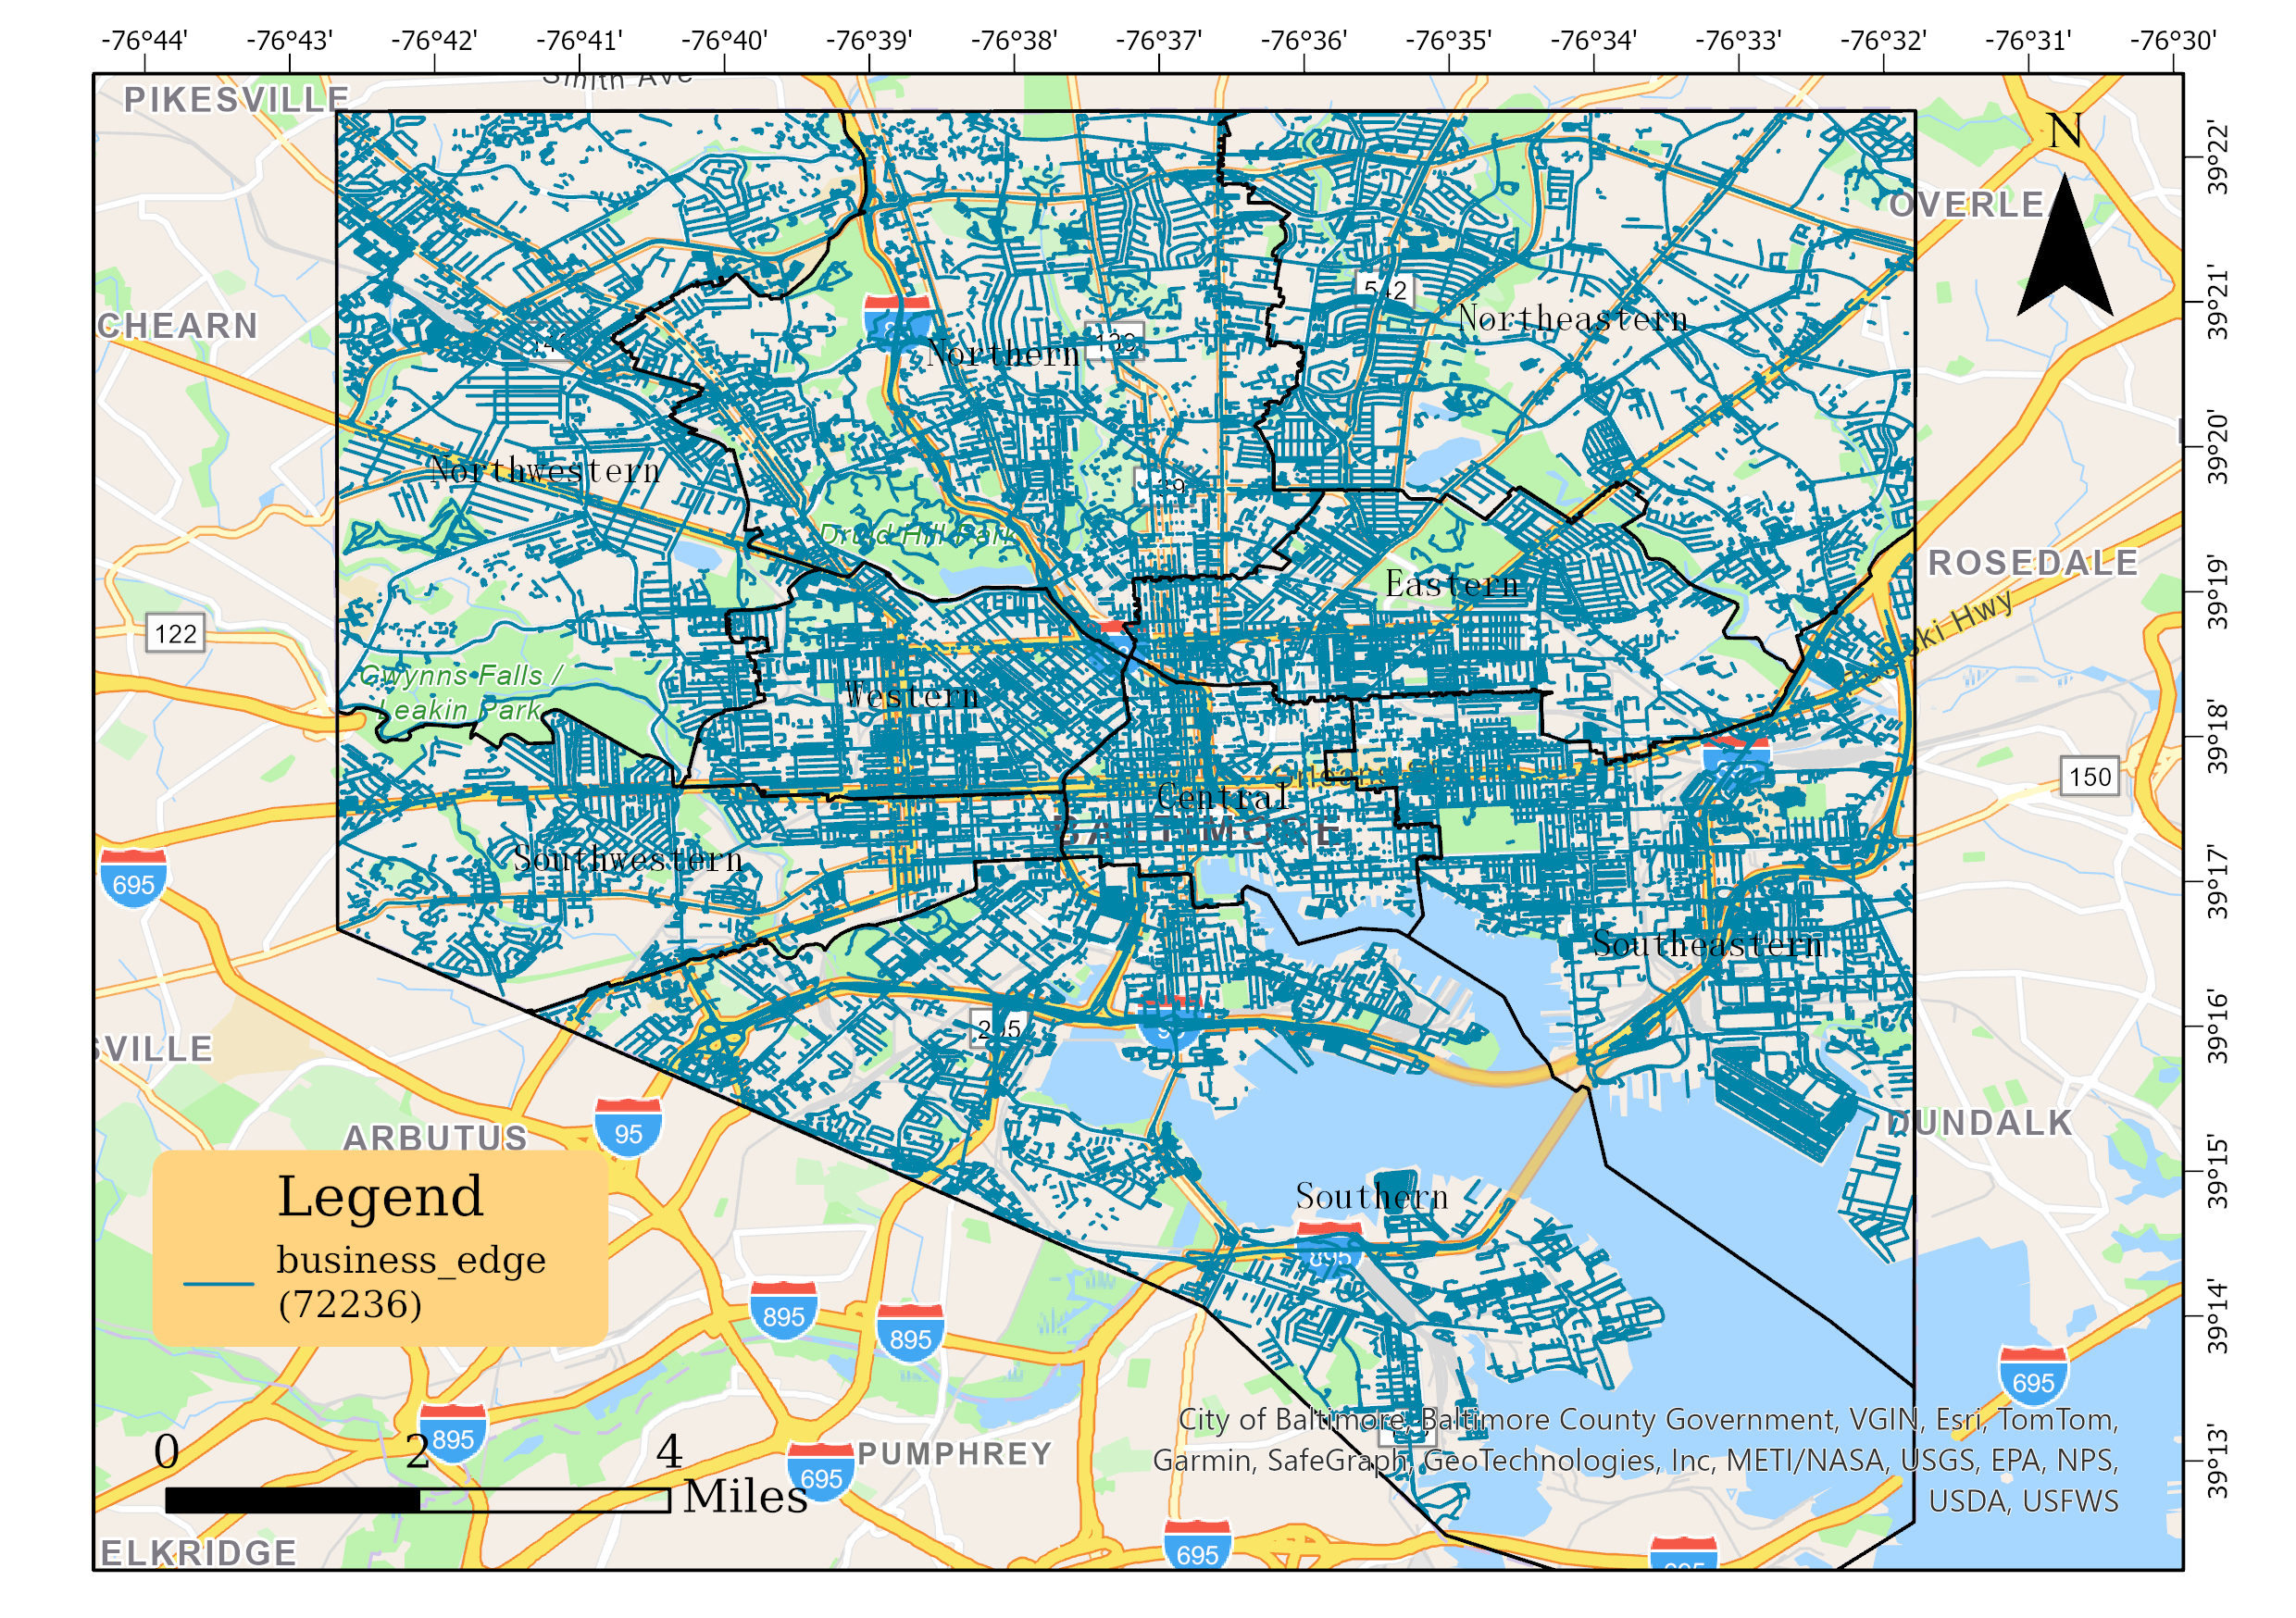
\includegraphics[width=\linewidth]{figures/business.jpg}
\end{minipage}%
\begin{minipage}{0.3\textwidth}
    \centering
    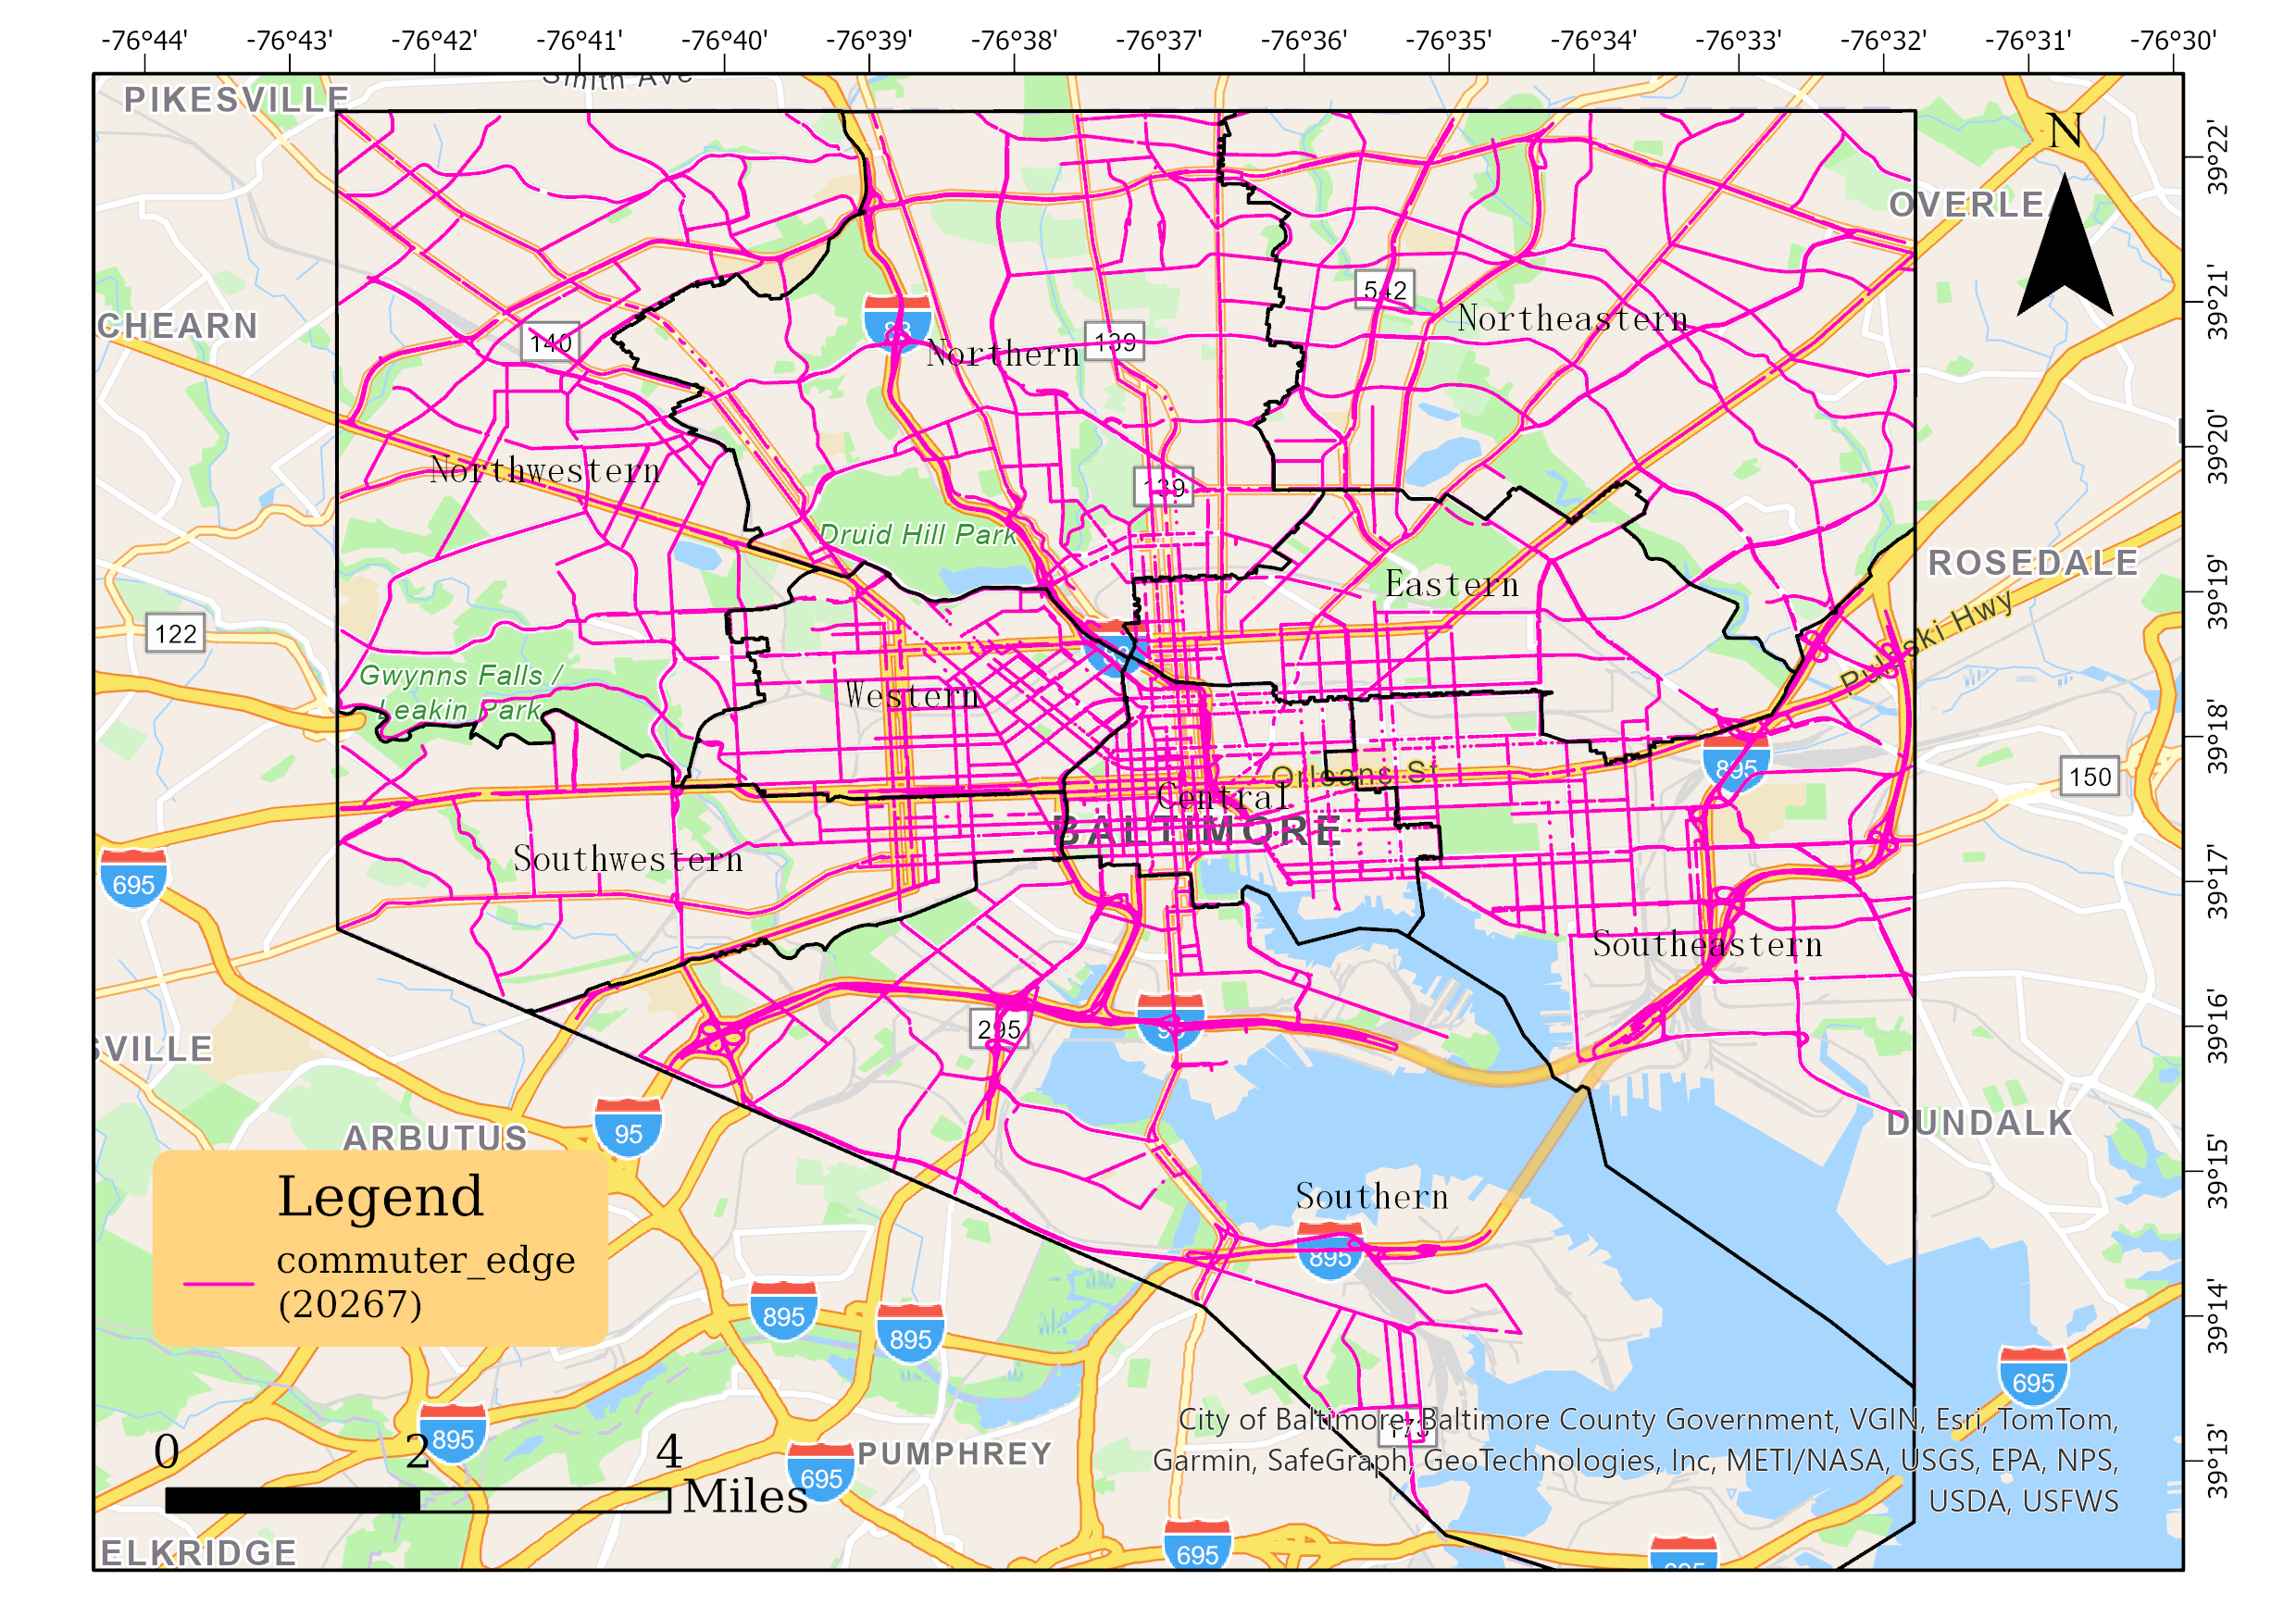
\includegraphics[width=\linewidth]{figures/commuter.jpg}
\end{minipage}%
\begin{minipage}{0.3\textwidth}
    \centering
    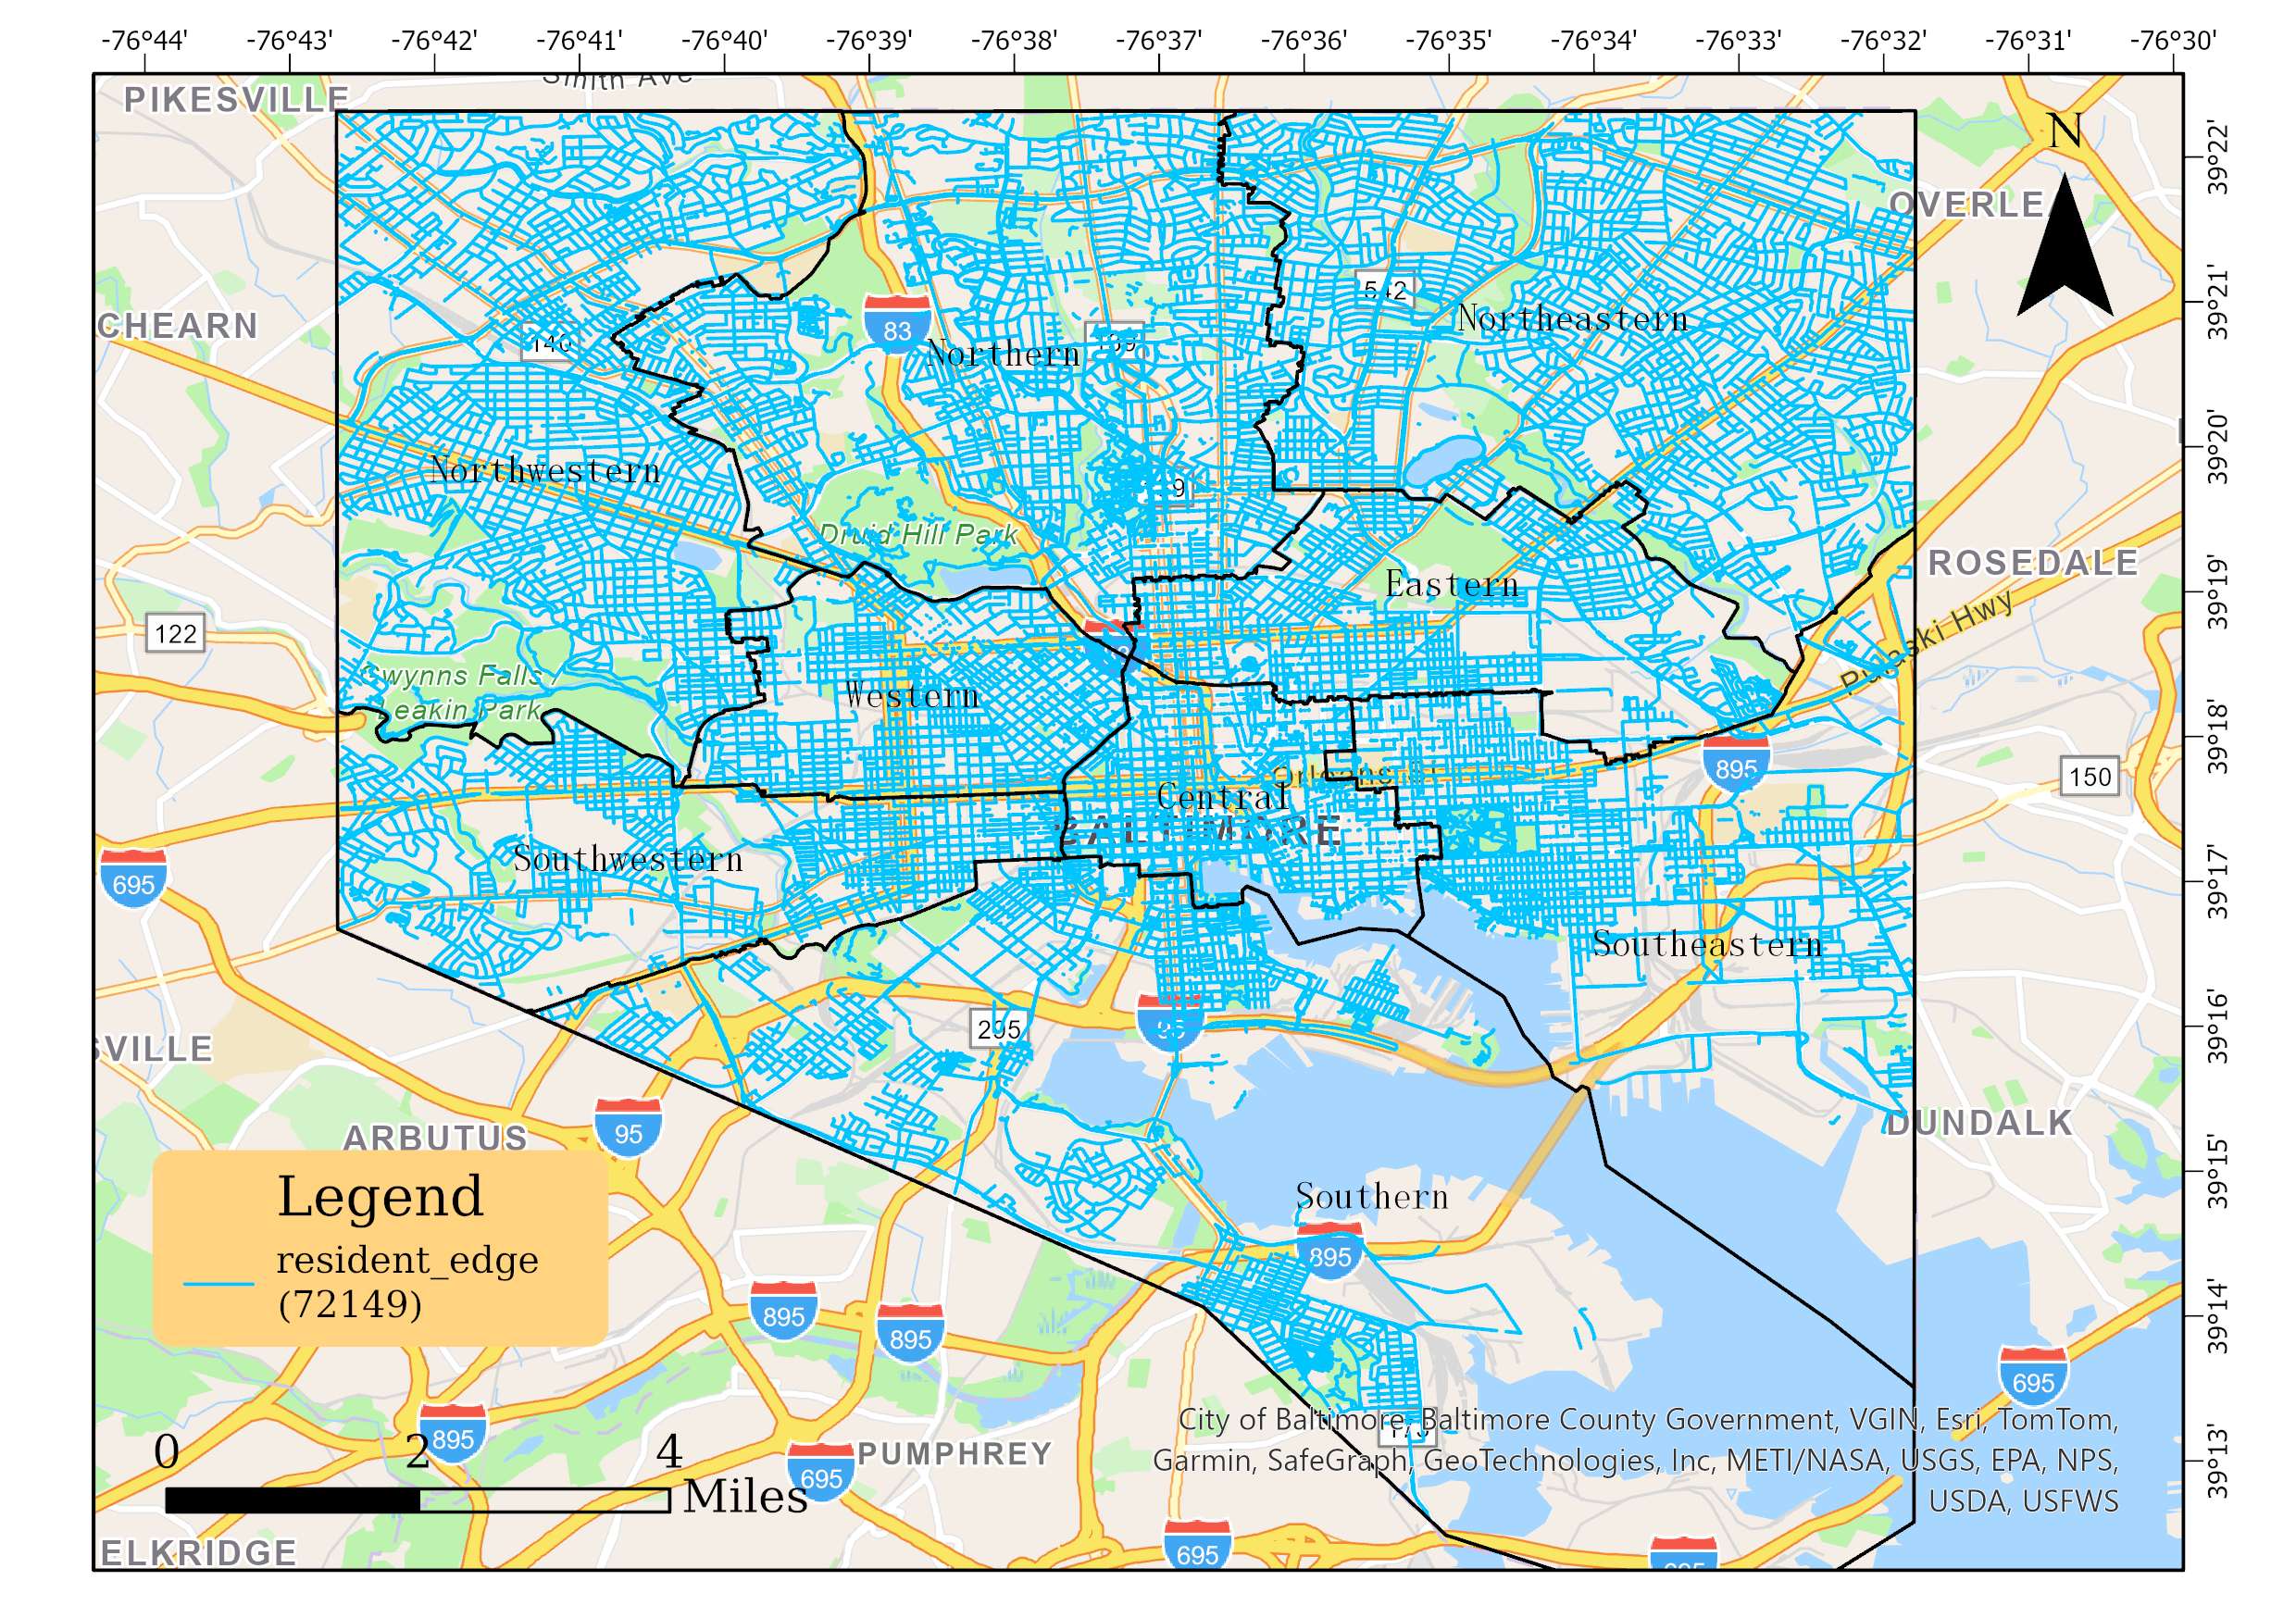
\includegraphics[width=\linewidth]{figures/resident.jpg}
\end{minipage}

\vskip 0.5cm

\begin{minipage}{0.3\textwidth}
    \centering
    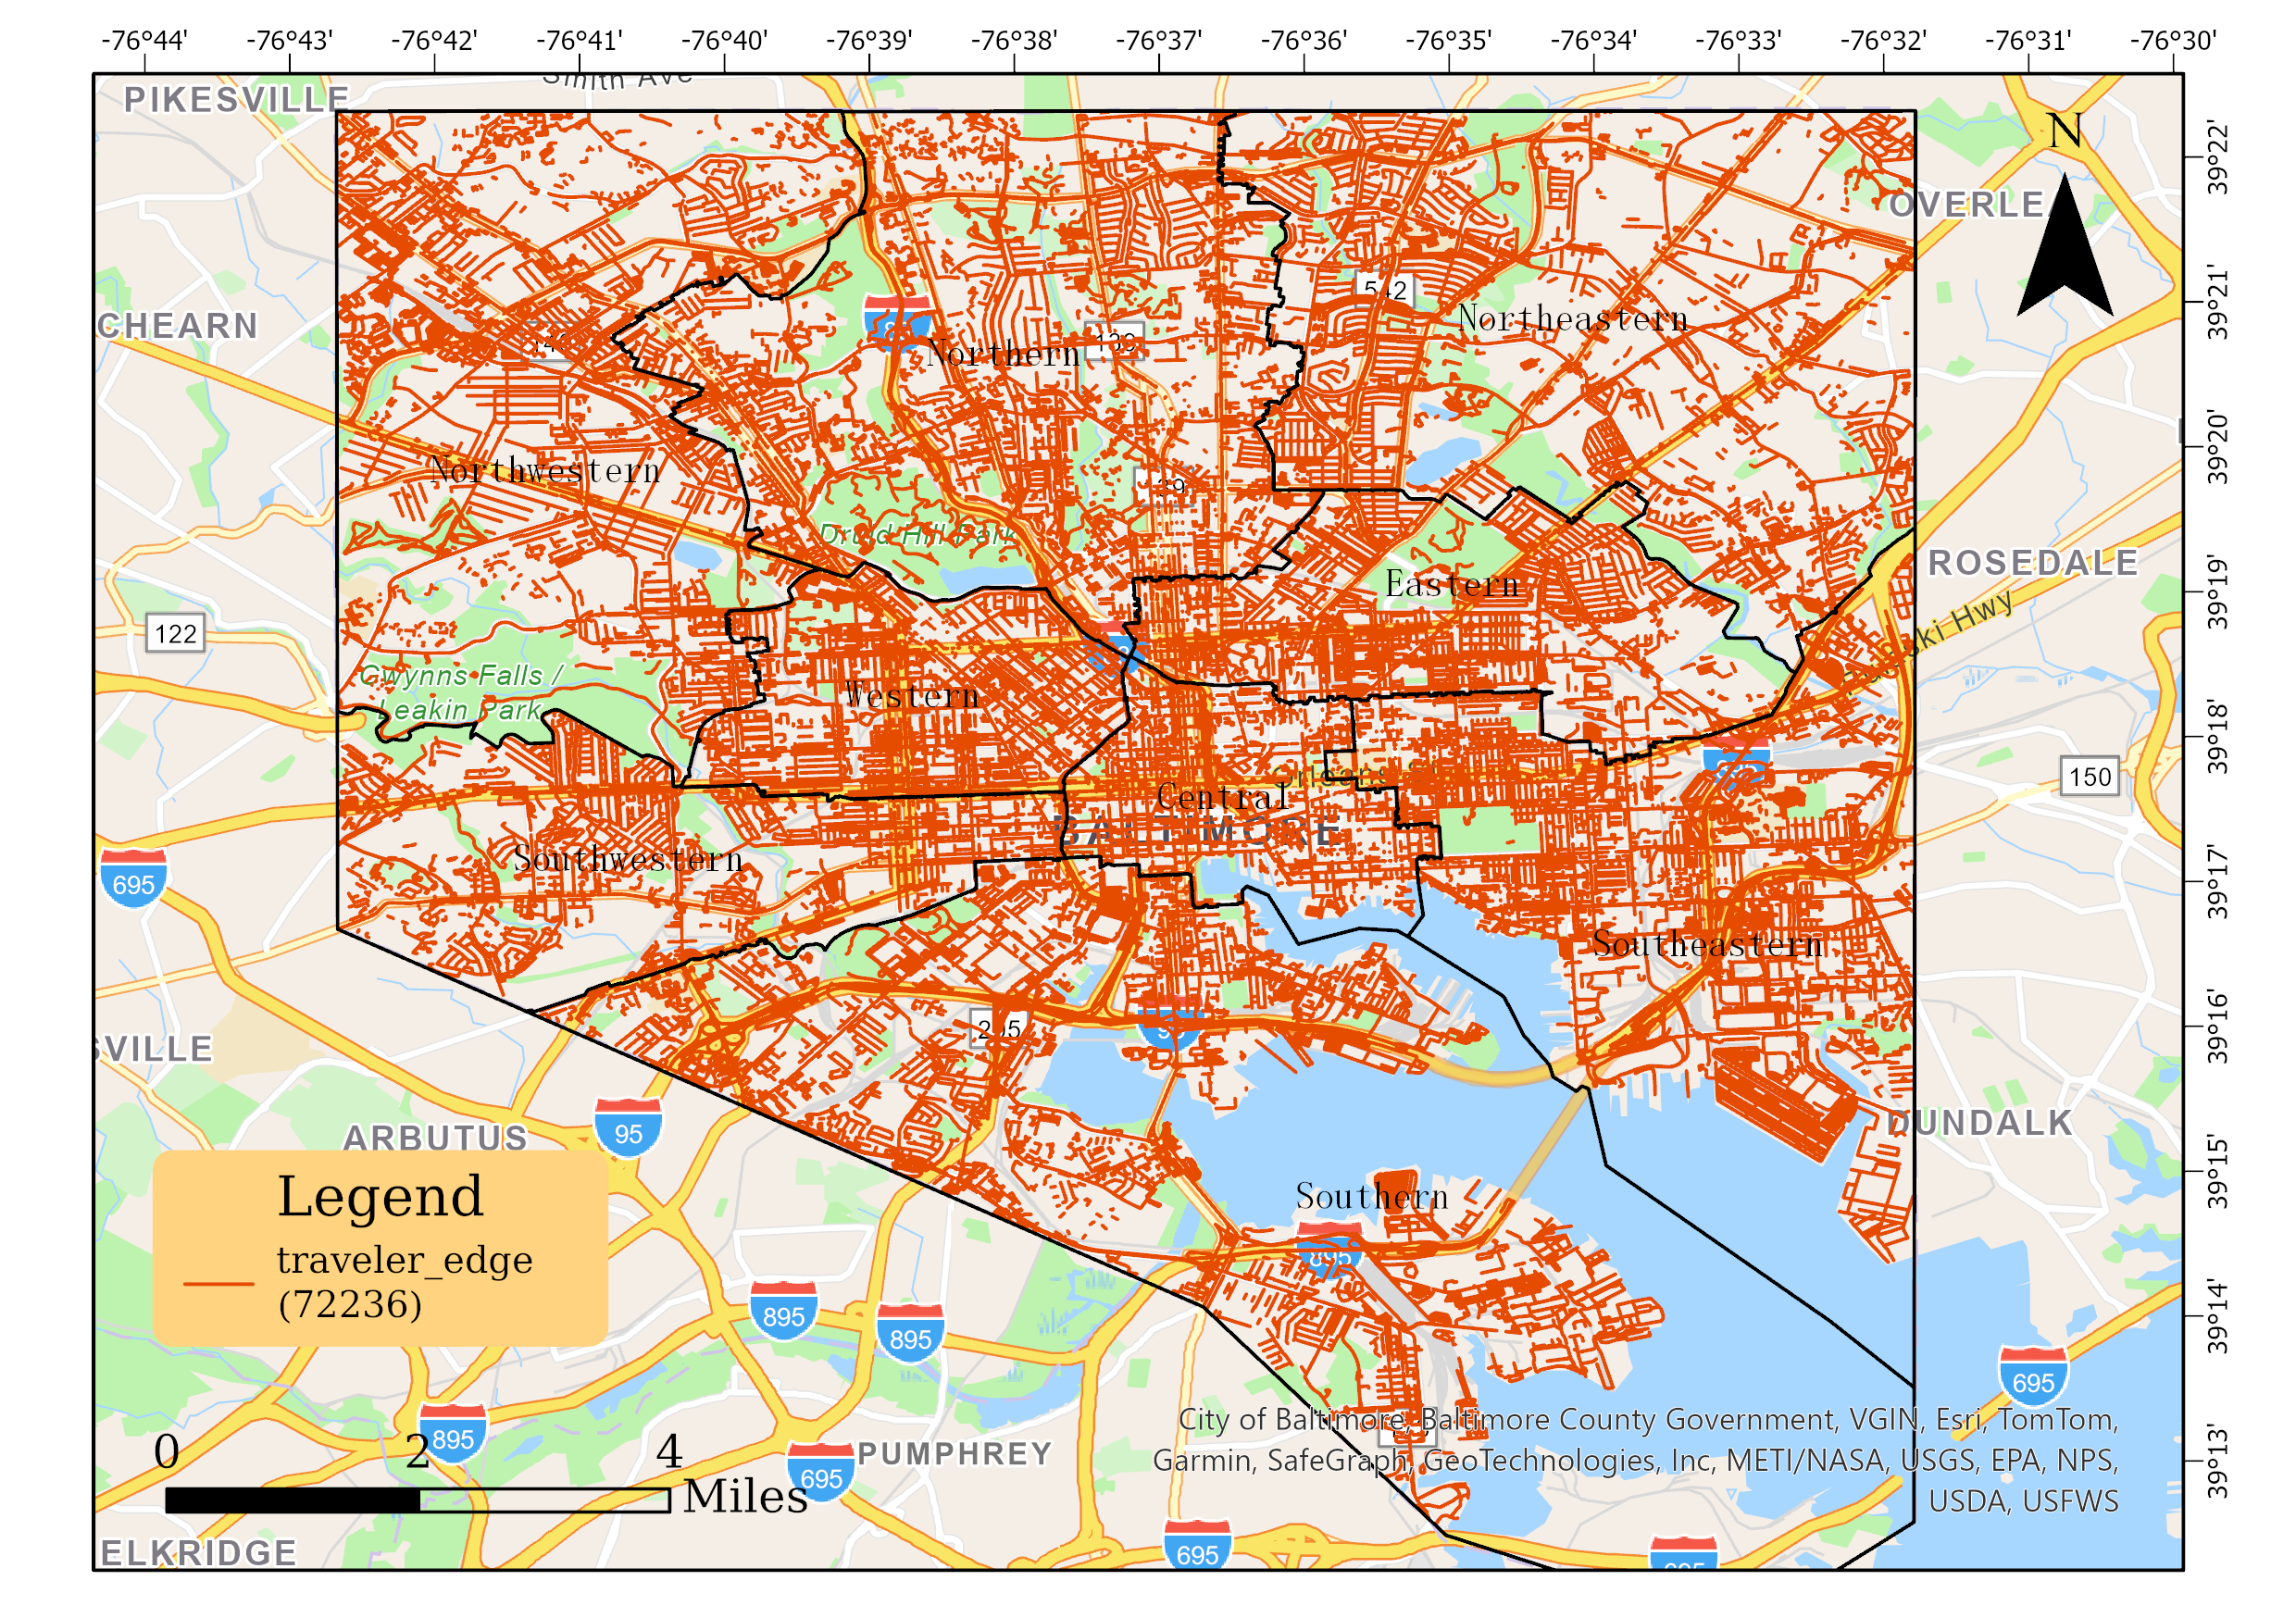
\includegraphics[width=\linewidth]{figures/traveler.jpg}
\end{minipage}%
\begin{minipage}{0.3\textwidth}
    \centering
    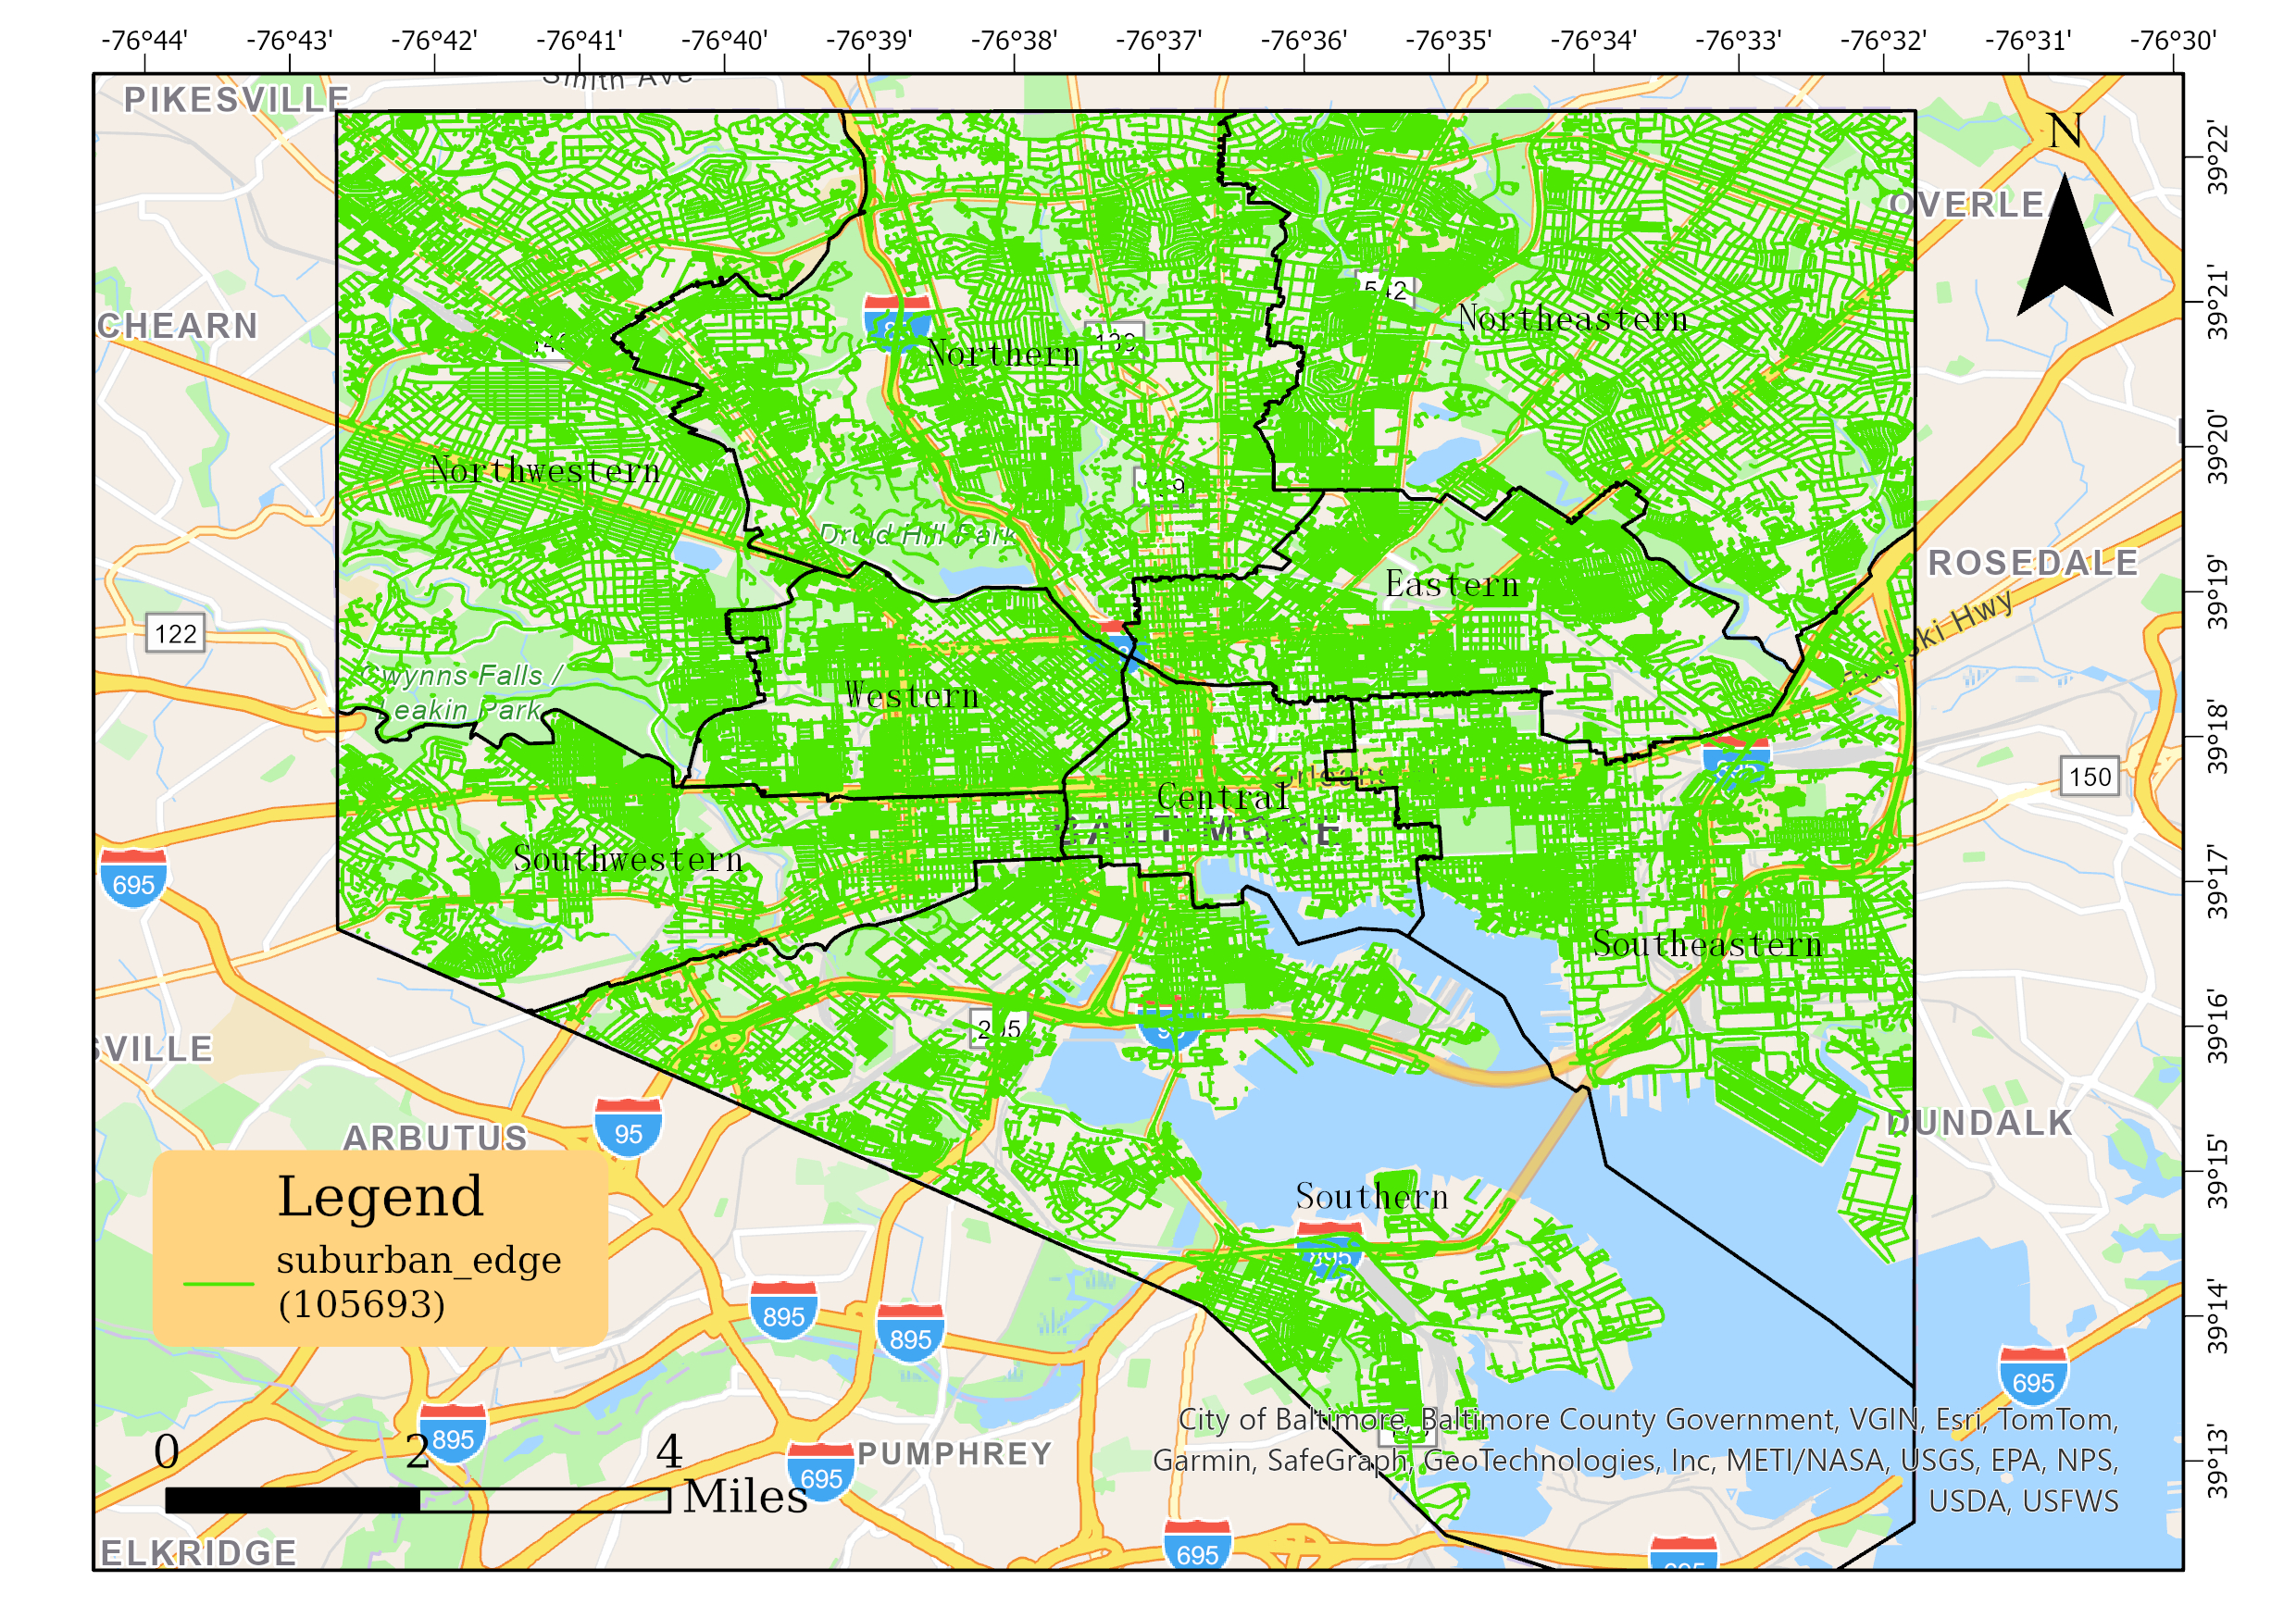
\includegraphics[width=\linewidth]{figures/suburban.jpg}
\end{minipage}%
\begin{minipage}{0.3\textwidth}
    \centering
    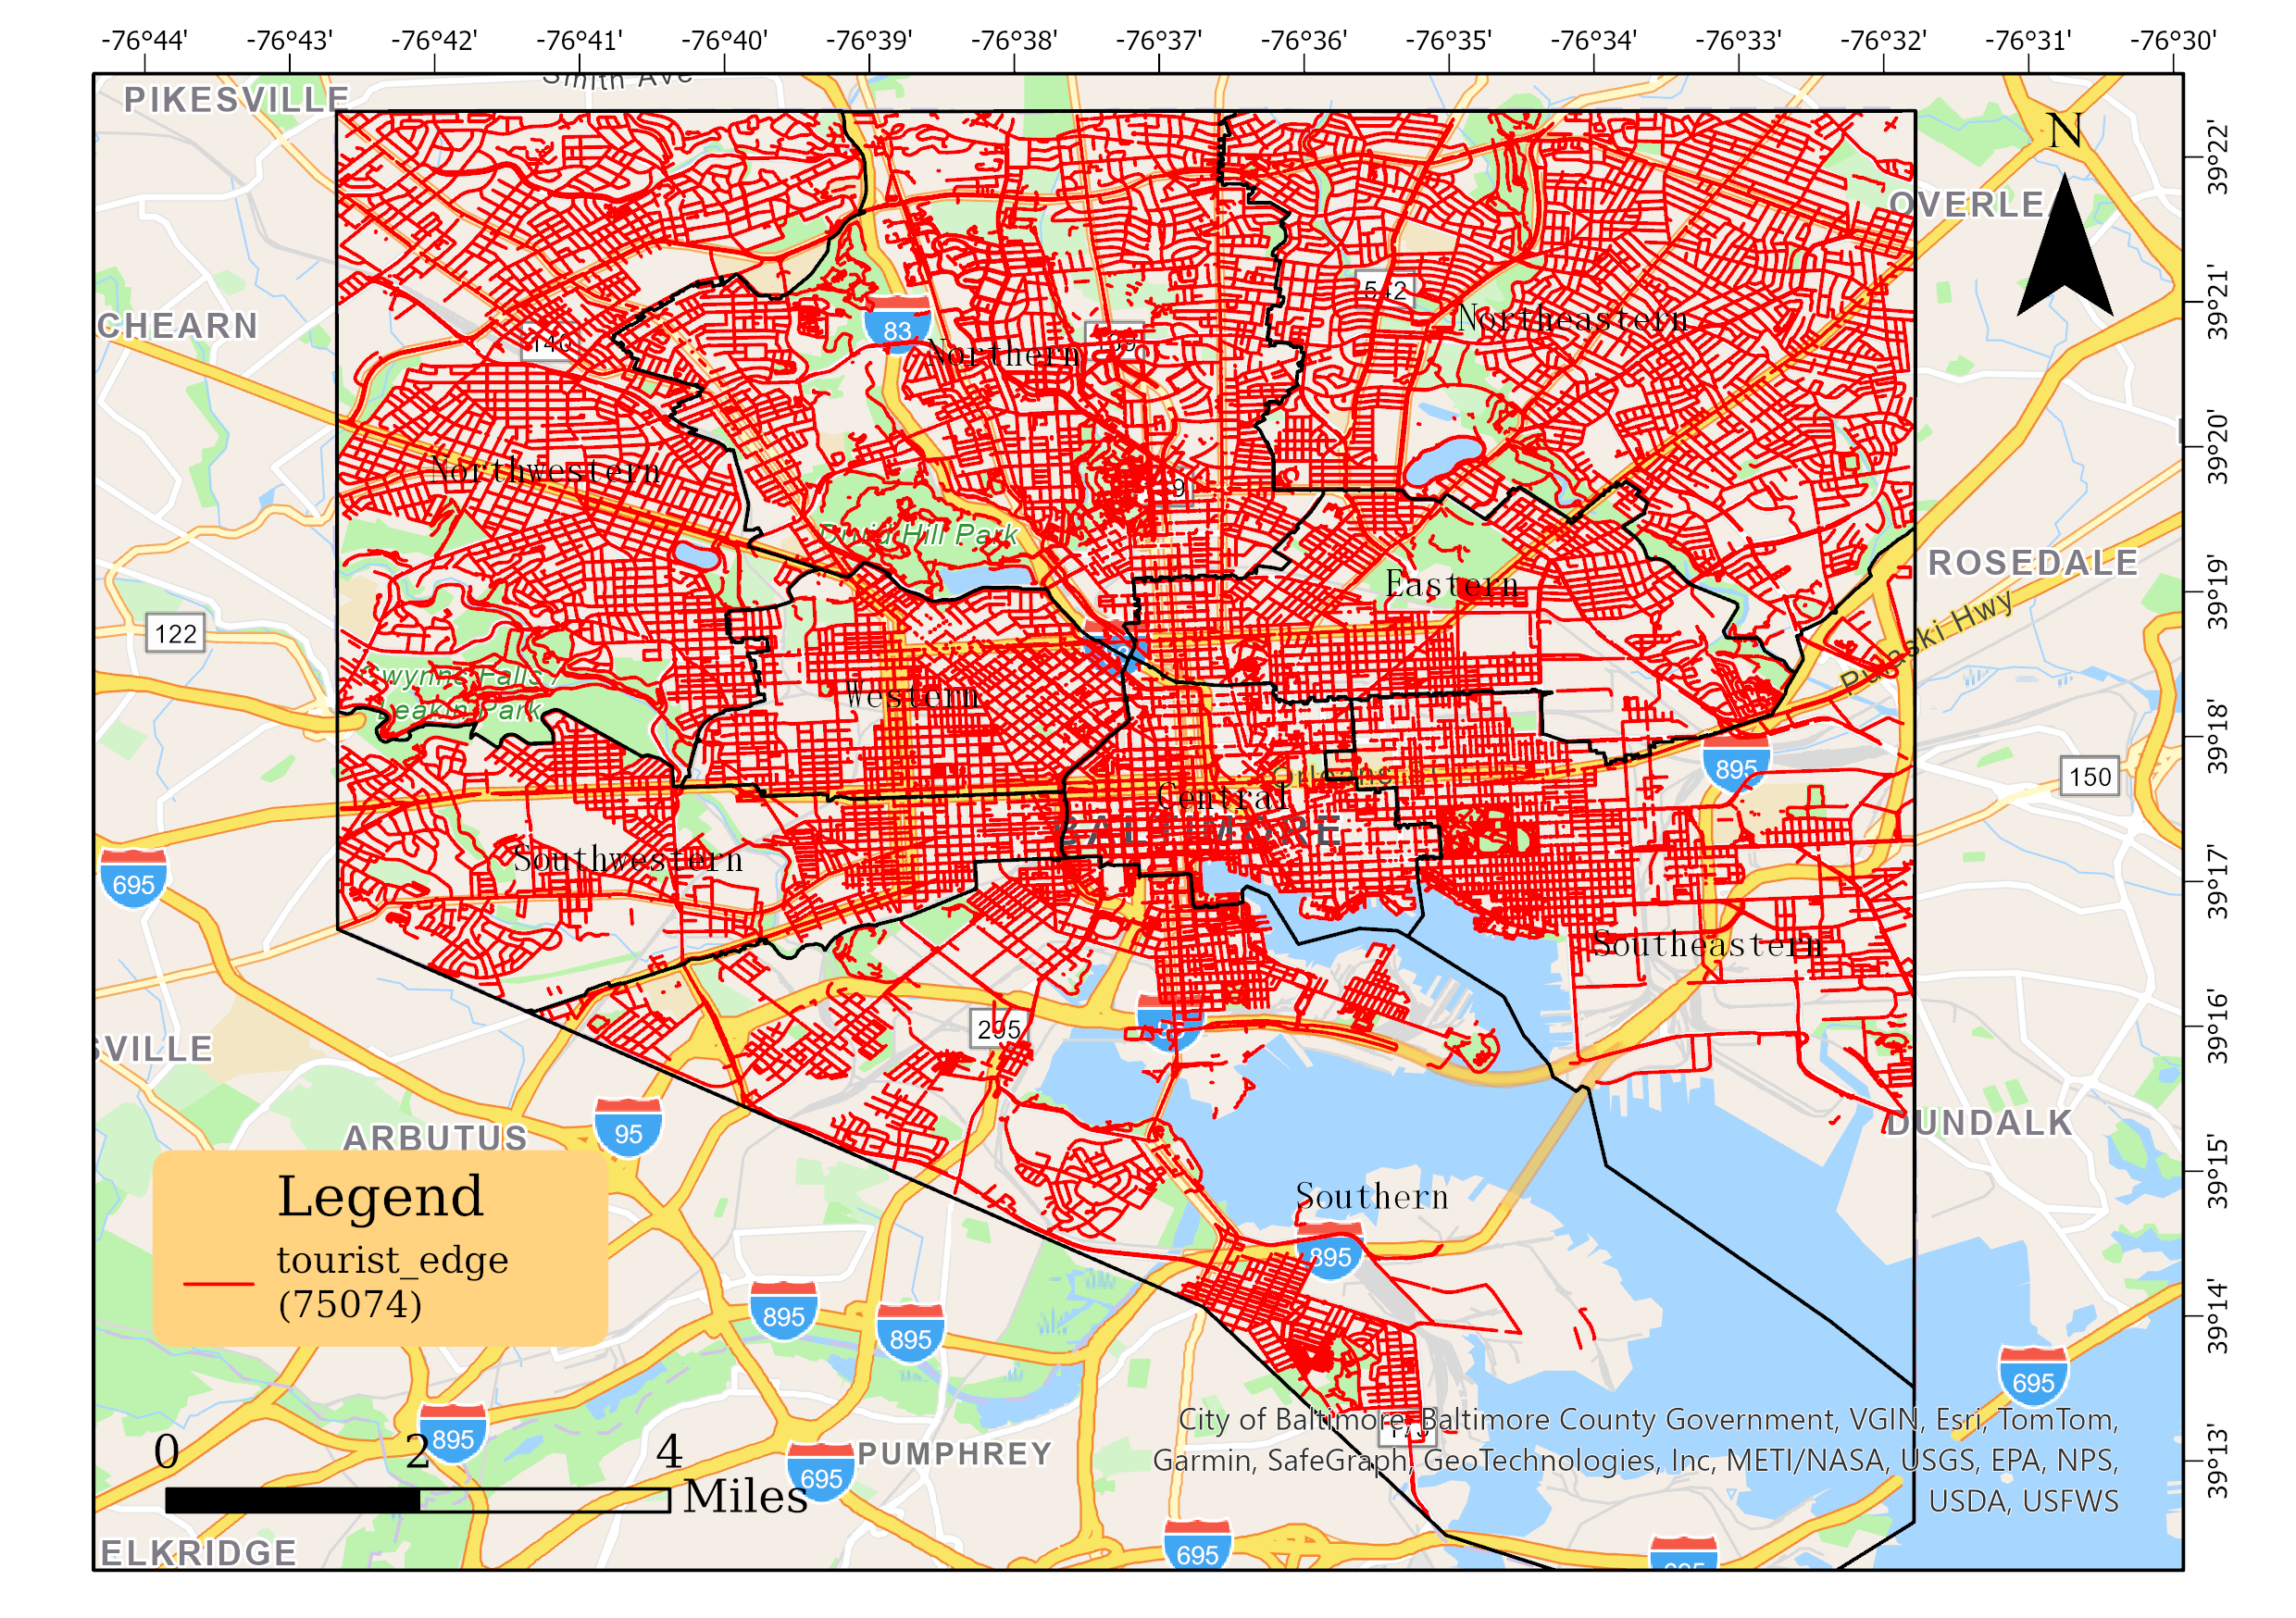
\includegraphics[width=\linewidth]{figures/tourist.jpg}
\end{minipage}

\caption{Road Network Mapping Based on Stakeholder Preferences}
\label{fig:3x2_images}
\end{figure}




Based on the classification, road network maps tailored to stakeholder preferences can be generated to identify transportation needs and network deficiencies. For example, in the southern region, insufficient roads for tourists and residents necessitate enhancing pedestrian pathways, cycling lanes, and public transit near tourist areas, as well as improving residential road connectivity.

Considering local cultural, tourism, and economic goals, road network expansion or optimization may be required. For instance, if the region focuses on tourism development, measures like adding roads to attractions, improving tourist zone facilities, and enhancing road quality and accessibility can attract more visitors and boost economic growth. Simultaneously, improving residential road networks and public transit will enhance residents' quality of life and satisfaction with government services.


\subsubsection{Traffic Zone Construction}

Traffic Analysis Zones (TAZs) are geographic areas constructed based on the road network and are used for traffic planning, management, and research. They are the fundamental analytical units of urban or regional transportation systems and help in understanding and managing complex traffic patterns.

\vspace{-5mm}
\begin{itemize}
    \item \textbf{Generation Method:}The Voronoi\cite{edelsbrunner1985voronoi} polygon \cite{boeing2024} is a spatial partitioning method that divides a plane into multiple regions, each corresponding to a generating point (such as a road node). Any point within a region has a shorter distance to the corresponding generating point than to any other generating point.

    \item \textbf{Mathematical Expression:} Given a set of generating points \( P = \{p_1, p_2, \dots, p_n\} \), the region \( V(p_i) \) of a Voronoi polygon is defined as:
    \vspace{-2mm}
    \[
V(p_i) = \{ x \in \mathbb{R}^2 \mid d(x, p_i) \leq d(x, p_j) \, \text{for all} \, j \neq i \}
\]
\vspace{-3mm}
    where \( d(x, p_i) \) is the distance from point \( x \) to the generating point \( p_i \).

    The distance-based partitioning method aligns with the basic requirements of  zones, where travel distances within a zone are relatively short. Moreover, the Voronoi polygon generation algorithm is computationally efficient, making it suitable for large-scale node data\cite{openstreetmap2025}.

\end{itemize}

    \begin{figure}[htbp]
        \centering
        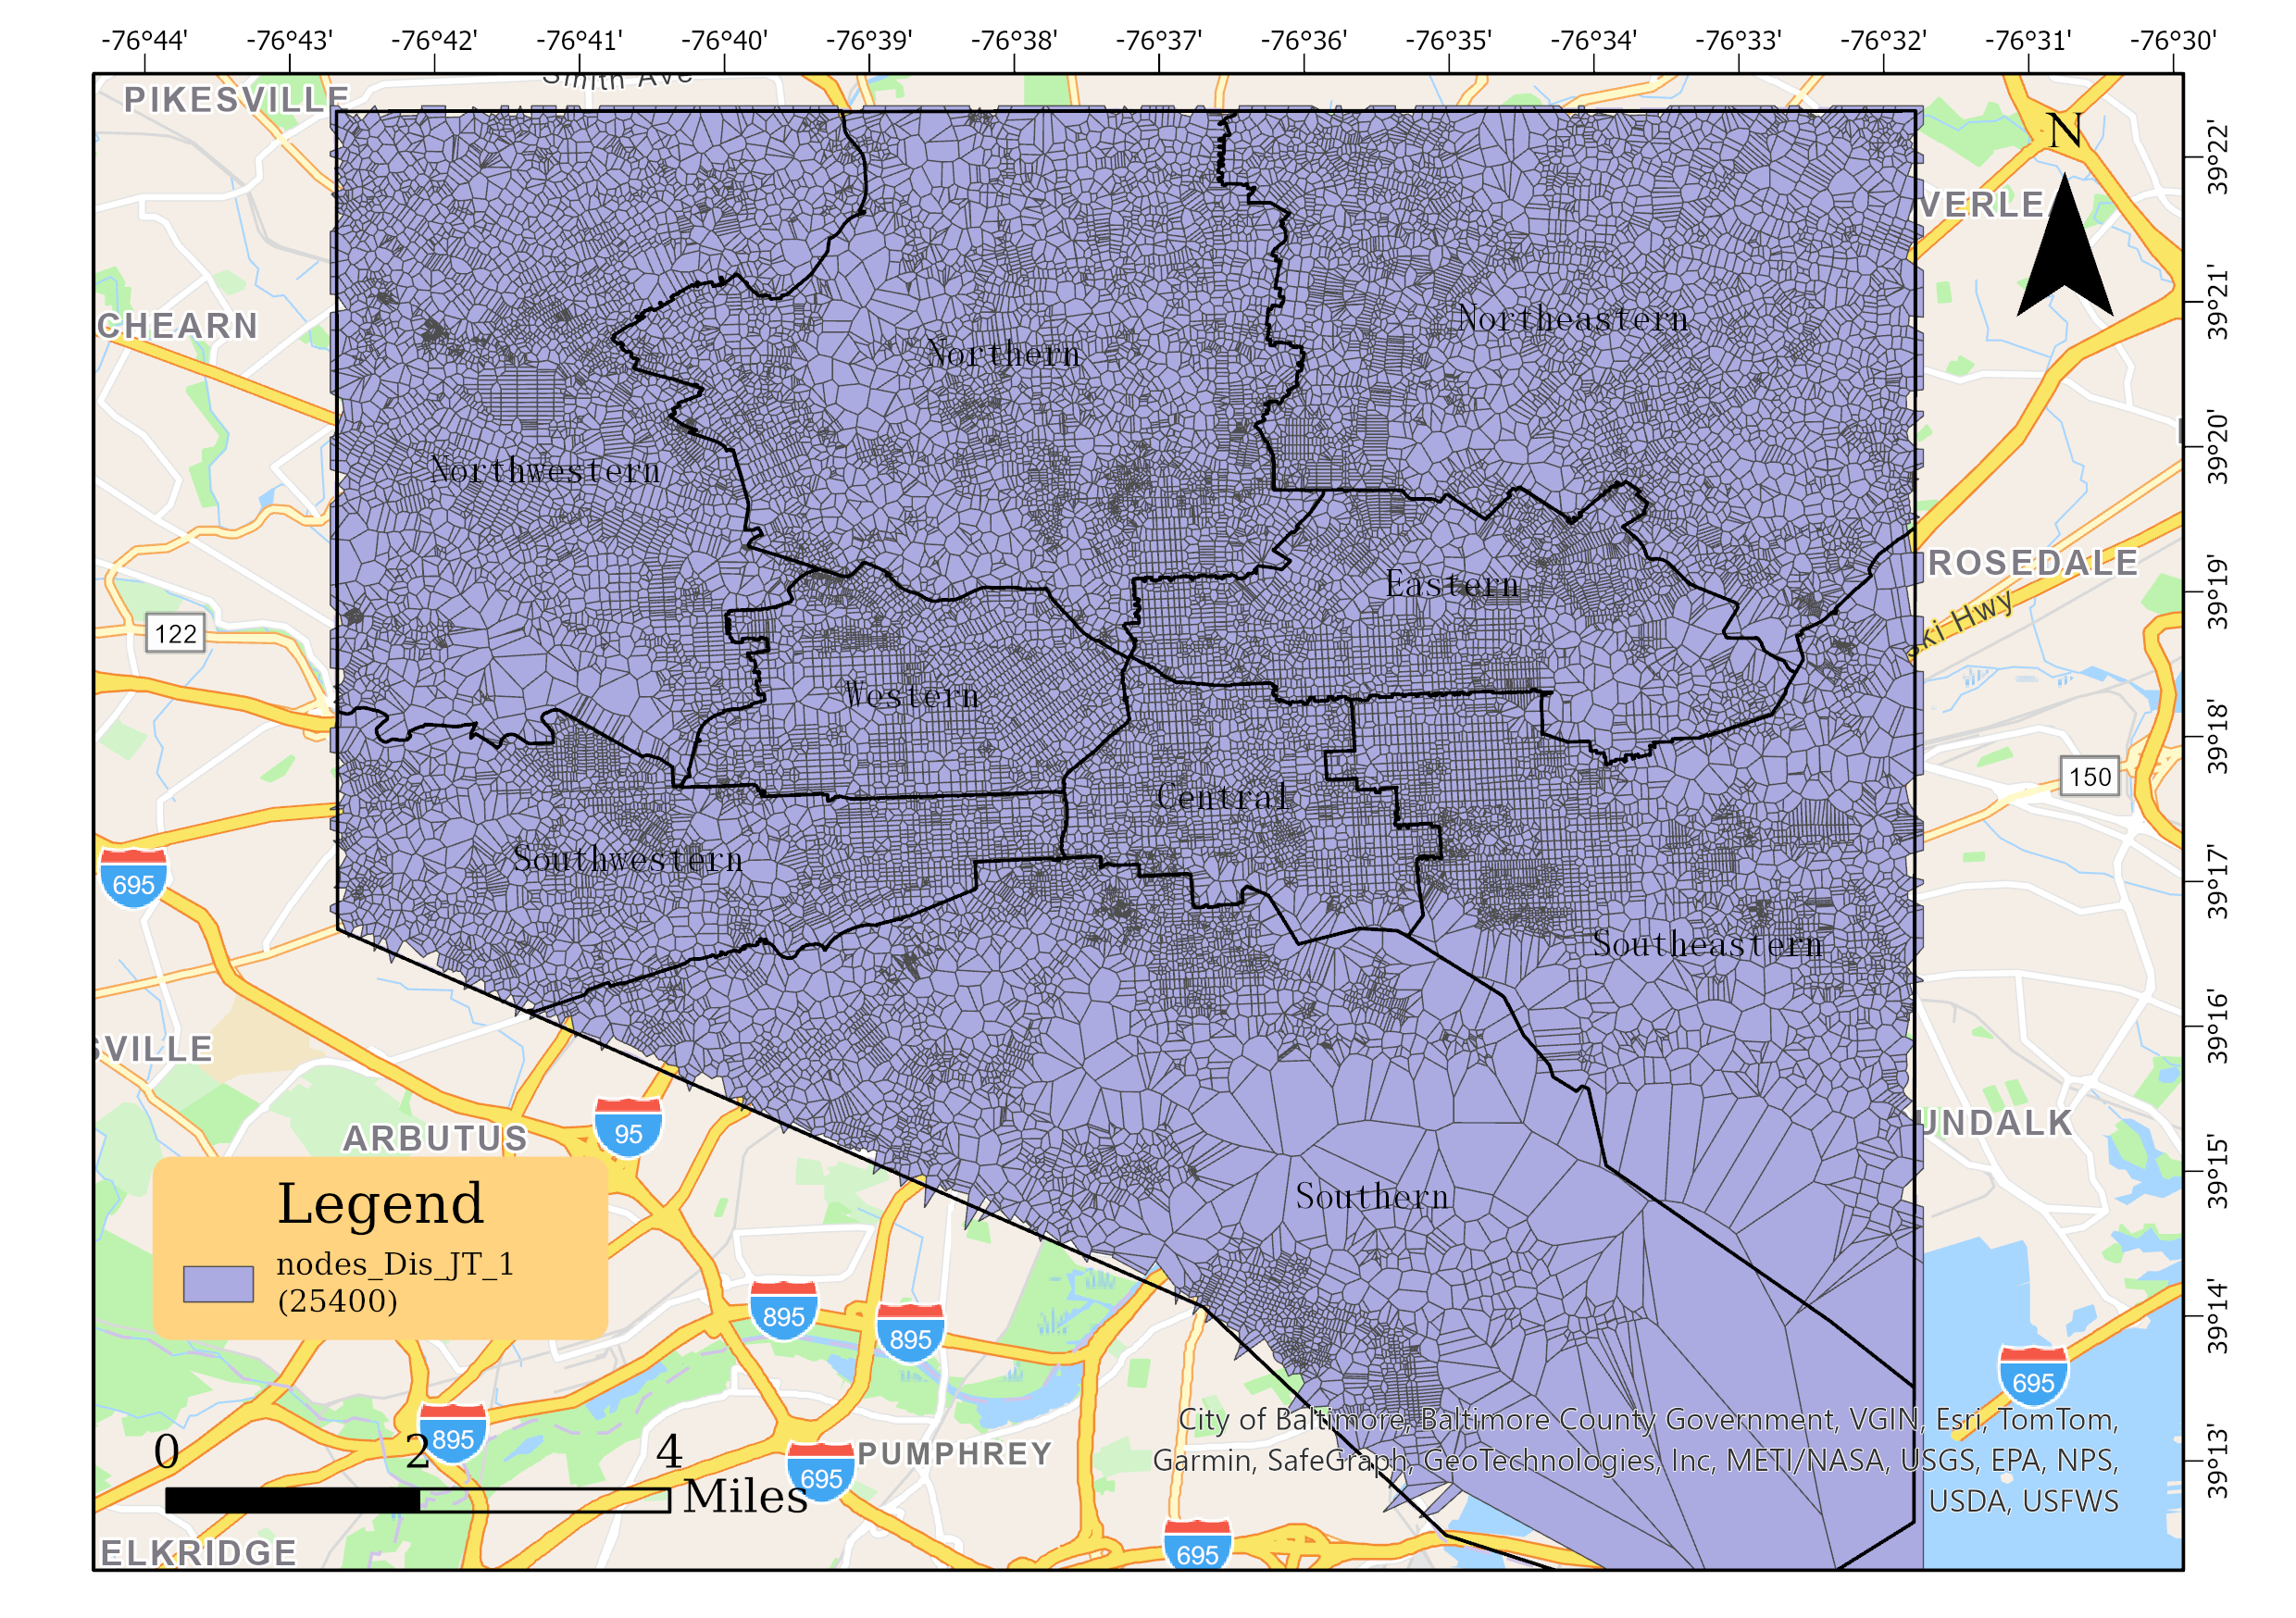
\includegraphics[width=0.685\linewidth]{figures/nodes.jpg}
        \caption{Example of Traffic Zone Partitioning}
        \label{fig:enter-label}
    \end{figure}


\subsubsection{Regional Transportation Accessibility Evaluation Based on Traffic Zones}

In urban transportation planning and management, evaluating regional transportation accessibility is a crucial task. This section explores how to evaluate regional transportation accessibility based on Traffic Analysis Zones (TAZs), which serve as the basic analytical units of urban or regional transportation systems, aiding in the understanding and management of complex traffic patterns.

We use three key formulas to quantify transportation accessibility. Formula 1 calculates the average area of each traffic zone, reflecting the scale of the zones. Formula 2 calculates the number of traffic zones per unit area, assessing the density of the traffic zones. These two indicators provide insight into the spatial distribution characteristics of the traffic zones.


\begin{itemize}
    \item \textbf{Formula 1:} To calculate the average area of each traffic zone, which reflects the scale of the traffic zones:
    \[
    \text{Average Traffic Zone Area} = \frac{\text{Total Area of Traffic Zones}}{\text{Number of Traffic Zones}}
    \]

    \item \textbf{Formula 2:} To calculate the number of traffic zones per unit area, which evaluates the density of traffic zones:
    \[
    \text{Traffic Zones per Square Kilometer} = \frac{\text{Number of Traffic Zones}}{\text{Area of the Region}}
    \]

    \item \textbf{Formula 3:} To evaluate the transportation accessibility of each region:
    \[
\begin{split}
\text{Accessibility} = &\left( 1 - \ln \left( \frac{\text{Average Traffic Zone Area}}{\text{Maximum Average Traffic Zone Area}} \right) \right) \\
&\times \left( \frac{\text{Average Traffic Zones per Square Kilometer}}{\text{Maximum Average Traffic Zones per Square Kilometer}} \right)
\end{split}
\]

\end{itemize}


 We have compiled statistics on the number and area of zones in different administrative regions:

\begin{table}[htbp]
\centering
\begin{tabular}{lccc}
\toprule
\textbf{District Name} & \textbf{Number of Traffic Zones} & \textbf{Traffic Zones per Square Kilometer} & \textbf{Accessibility} \\
\midrule
Western       & 1115 & 116 & 1.05 \\
Southeastern  & 2905 & 92  & 0.72 \\
Northwestern  & 3597 & 109 & 0.95 \\
Central       & 1509 & 184 & 2.13 \\
Eastern       & 1939 & 140 & 1.86 \\
Northern      & 4305 & 138 & 1.85 \\
Southern      & 3470 & 59  & 0.44 \\
Northeastern  & 3962 & 112 & 0.82 \\
Southwestern  & 2264 & 136 & 1.00 \\
\bottomrule
\end{tabular}
%\caption{Traffic Zones and Accessibility by District}
\label{tab:traffic_zones}
\end{table}


As the area increases, transportation becomes less efficient, and as the number of zones decreases, transportation becomes more sparse.

By analyzing the geographic locations and accessibility indicators of various regions, we can assess the public transportation conditions of each area. This will also serve as the basis for future public transportation development proposals.

Identifying regions with low transportation accessibility provides a foundation for subsequent public transportation planning. Through the analysis of traffic zone quantity and area across different administrative regions, we obtain a series of data. These results demonstrate differences in transportation accessibility between regions. For example, the Western region has an accessibility index of 1.05, indicating a relatively dense transportation network, while the Southern region has an accessibility index of only 0.44, suggesting a sparser transportation network that may require further improvements and investments in transportation infrastructure.


\subsection{ Traffic Flow Road Network Based on Topological Structure}

\subsubsection{Algorithm: Topology-Based Traffic Flow Road Network}

For traffic flow data, the network is not simply composed of edge or node data. Instead, the road network is constructed based on its topological structure. The algorithm for constructing a traffic flow road network is described as follows:

\textbf{(1) Data Parsing}

\begin{itemize}
    \item \textbf{Read CSV File}: Use Python's "csv" module to open and read the CSV file.  

    \item \textbf{Line-by-Line Parsing}: Parse the content of the file line by line and store each record. 

    \item \textbf{Extract Nodes and Road Attributes}:For each record, extract the fields node start and node(s) end, which represent the starting and ending nodes of the road.  

    \item \textbf{Extract Additional Road Attributes}:Fields such as "Road Name", "Functional Class", etc., are extracted for later use in establishing topological relationships and network analysis.
\end{itemize}


\textbf{(2) Identification of Nodes and Edges}

\begin{itemize}
    \item \textbf{Identify Nodes}:Create a set of nodes to store all unique node identifiers.  

    \item \textbf{Identify Edges}:Create a list of edges to store all road segments.  

    \item \textbf{Extract Nodes and Road Attributes}:For each record, extract the fields node start and node(s) end, which represent the starting and ending nodes of the road.  

\end{itemize}

\textbf{(3) Establishment of Topological Relationships}
\vspace{-5mm}

\begin{itemize}
    \item \textbf{Topological Relationship Construction}:
        \begin{itemize}
            \item Use a graph data structure to represent the road network.  

            \item Add identified nodes as nodes in the graph.  

            \item Add identified edges as edges in the graph, with corresponding attributes.  
        \end{itemize}
        

    \item \textbf{Handling Multiple Types of Connections}:
        \begin{itemize}
            \item For \textbf{one-to-one} relationships, directly add one edge in the graph. 

            \item For \textbf{one-to-many} relationships, add multiple edges from a single starting node to different ending nodes.  

            \item For \textbf{many-to-one} relationships, add edges from multiple starting nodes to a single ending node. 

            \item For \textbf{many-to-many} relationships, add multiple edges to represent complex connection patterns.
        \end{itemize}  

\end{itemize}

\vspace{-6mm}
\textbf{(4) Connectivity Check}
\vspace{-5mm}

\begin{itemize}
    \item Ensure that all nodes and edges are connected, with no isolated nodes or edges.

    \item Use topology check tools (e.g., ArcGIS topology check tools) to detect and resolve issues. 

\end{itemize}



\vspace{-5mm}
\textbf{(5) Consistency Check}
\vspace{-3mm}

\begin{itemize}
    \item Ensure that the topological relationships in the road network align with reality, avoiding duplicate edges or nodes.

   \begin{figure}[htbp]
       \centering
       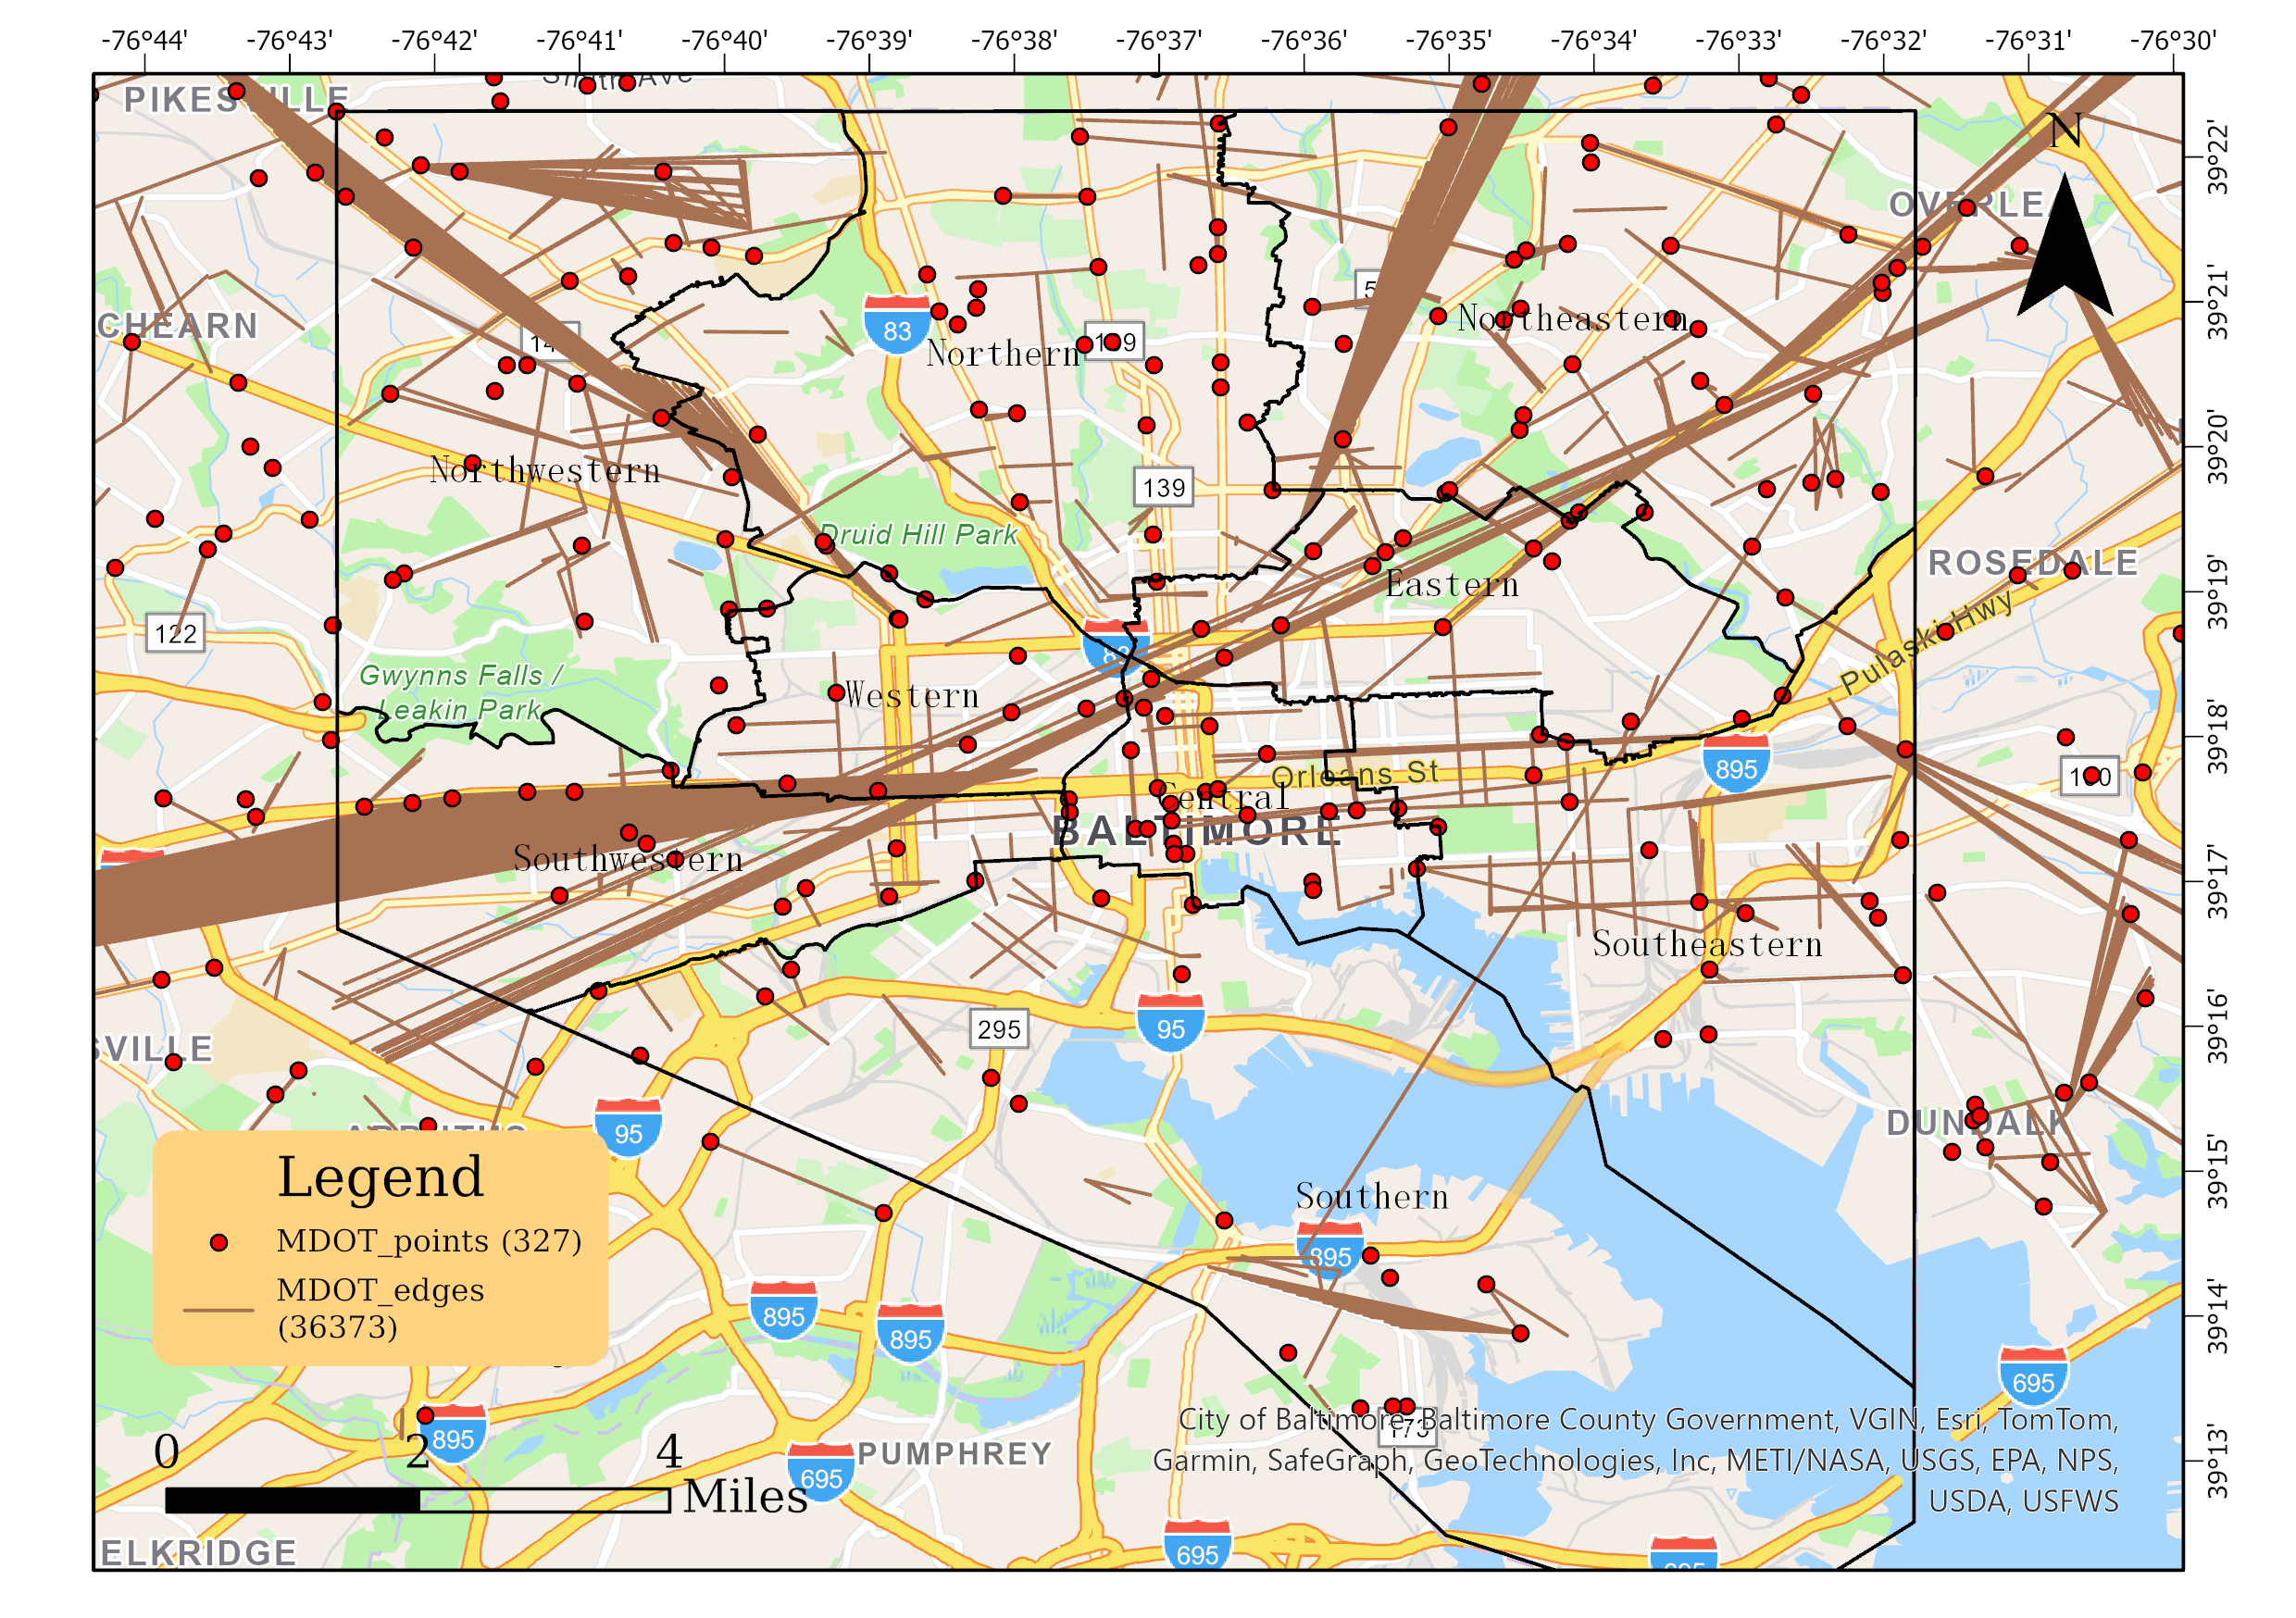
\includegraphics[width=0.75\linewidth]{figures/MOOT.jpg}
       \caption{Traffic Flow Road Map}
       \label{fig:enter-label}
   \end{figure}

\end{itemize}

\subsubsection{Road Network Attributes}

The roads in the network\cite{mdot2025} possess the following attributes, which are analyzed and organized:

\textbf{(1) Traffic Classification and Functional Indicators}

\begin{itemize}
    \item \textbf{Rural / Urban}: Indicates the type of area the road is located in, affecting traffic patterns and planning. 

    \item \textbf{Functional Class Code / Functional Class}:Defines the functional classification of the road, such as major highways, minor highways, etc.
\end{itemize}




\textbf{(2) Traffic Flow Indicators}


\begin{table}[ht]
\centering
\begin{tabular}{>{\centering\arraybackslash}p{4cm} >{\centering\arraybackslash}p{8cm}} % 控制列宽并使内容居中
\toprule
\textbf{Traffic Flow Indicator} & \textbf{Description} \\
\midrule
\textbf{AADT (Annual Average Daily Traffic)} & Measures the average daily vehicle count on the road, indicating traffic volume. \\
\textbf{AAWDT (Annual Average Weekday Traffic)} & Measures the annual average traffic volume on weekdays, excluding weekends. \\
\textbf{AADT by Vehicle Type} & Measures the AADT for different vehicle types \\
\bottomrule
\end{tabular}
\caption{Traffic Flow Indicators and Descriptions}
\label{tab:traffic_flow_indicators}
\end{table}


These values represent the annual average daily traffic volumes by different vehicle types, enabling the analysis of traffic composition.

\textbf{(3) Traffic Direction and Timing Indicators}

\begin{itemize}
    \item \textbf{Peak Hour Direction}:The dominant traffic direction during peak hours, essential for traffic management and signal control.  

    \item \textbf{North-East Split / South-West Split}:Distribution of traffic flow direction, assisting in understanding traffic flow patterns.
\end{itemize}

\textbf{(4) Traffic Efficiency and Impact Indicators}

\begin{itemize}
    \item \textbf{Average Vehicle Miles Traveled (AVMT)}:Measures the average vehicle miles traveled, reflecting the impact of traffic on the environment.    

    \item \textbf{K-Factor / D-Factor}:Statistical factors used to adjust traffic flow data, reflecting the distribution of traffic during peak hours.
\end{itemize}



\section{Construction of Transportation Network Models}

\subsection{Construction of Basic Network Model}

\textbf{(1) Definition of Nodes and Edge}
\vspace{-5mm}
\begin{itemize}
    \item \textbf{Nodes:}Key points in the transportation network, including road intersections, transportation hubs, bridges, tunnels, and other critical locations.

    \item \textbf{Edge:}The paths (road segments) connecting the nodes. Each edge may include the following attributes:
        \begin{itemize}
            \item \textbf{Number of Lanes:}The number of lanes on the road segment.

            \item \textbf{Peak Hour Direction:}The primary direction of traffic flow during peak hours.

            \item \textbf{Traffic Flow Data:}Including AADT (Annual Average Daily Traffic), AAWDT (Annual Average Weekday Traffic), K-Factor, D-Factor, and other related metrics.

            \item \textbf{Average Vehicle Miles Traveled (AVMT):}The average distance traveled by vehicles on the road segment.

            \item \textbf{Direction Distribution:}The distribution of traffic flow in terms of cardinal directions, such as North-East Split and South-West Split.
        \end{itemize}
\end{itemize}

\vspace{-5mm}
\textbf{(2) Edge Weight Adjustment}

Assign weights to each edge based on factors such as travel time, capacity, traffic volume, and other relevant characteristics.


\subsection{Custom Network Model Construction}

\textbf{Preferred Locations}

There are 90 types of locations, each offering different services to people. Different stakeholders have different preferences regarding these locations. Therefore, we consider the accessibility of various location types for different stakeholders, including urban residents, business owners, suburban residents, commuters, passthrough travelers, and tourists. The preferences for these locations by various stakeholders are summarized below:

\vspace{2mm}
\begin{longtable}{*{6}{c}}  % 改为c，表示每一列居中对齐
  \toprule
  \multicolumn{2}{c}{Residents} & \multicolumn{2}{c}{Entrepreneurs} & \multicolumn{2}{c}{Tourists} \\
  \cmidrule(lr){1-2} \cmidrule(lr){3-4} \cmidrule(lr){5-6}
  Venue & Preference & Venue & Preference & Venue & Preference \\
  \midrule
  \endfirsthead

  \toprule
  \multicolumn{2}{c}{Residents} & \multicolumn{2}{c}{Entrepreneurs} & \multicolumn{2}{c}{Tourists} \\
  \cmidrule(lr){1-2} \cmidrule(lr){3-4} \cmidrule(lr){5-6}
  Venue & Preference & Venue & Preference & Venue & Preference \\
  \midrule
  \endhead

  \midrule
  \multicolumn{6}{r}{Continued on next page} \\
  \endfoot

  \bottomrule
  \endlastfoot

  apartments       & 5 & commercial         & 5 & hotel              & 5 \\
  clinic           & 4 & industrial         & 4 & museum             & 5 \\
  college          & 4 & office             & 5 & park               & 4 \\
  hospital         & 4 & warehouse          & 4 & restaurant         & 5 \\
  house            & 4 & workshop           & 4 & tourist\_attractions &5 \\
  kindergarten     & 4 & central\_office     &5 & cathedral          &4 \\
  library          & 4 & government         &4 & chapel             &4 \\
  park             & 4 & retail             &4 & church             &4 \\
  school           & 5 & storage\_tank       &3 & mosque             &4 \\
  sports\_centre   &3  & manufacture        &4 & temple             &4 \\
  university       &4  &                    &   & synagogue          &4 \\
  \addlinespace[2pt]
                     &   &                    &   & castle             &4 \\
  \addlinespace[2pt]
                     &   &                    &   & ruins              &3 \\

\end{longtable}

 
\section{A Comprehensive Analysis of the Impact of Bridge Collapse on Traffic Networks}

\subsection{Local Analysis of Bridge Collapse}

In the wake of the Dundalk Bridge collapse, the Maryland Department of Transportation acted swiftly, arranging detour routes for those who would have ordinarily passed through Dundalk or the Curtis Bay/Hawkins Point area. To bolster local traffic flow, the outer loop of I-695 was closed and rerouted via Exit 1/Isolation Road (passing the Curtis Creek Bridge), with the loop remaining closed at Exit 1 (MD 173). While this initiative sought to mitigate the traffic pressure caused by the bridge collapse, the port area continued to experience substantial traffic challenges.

\begin{figure}[htbp]
    \centering
    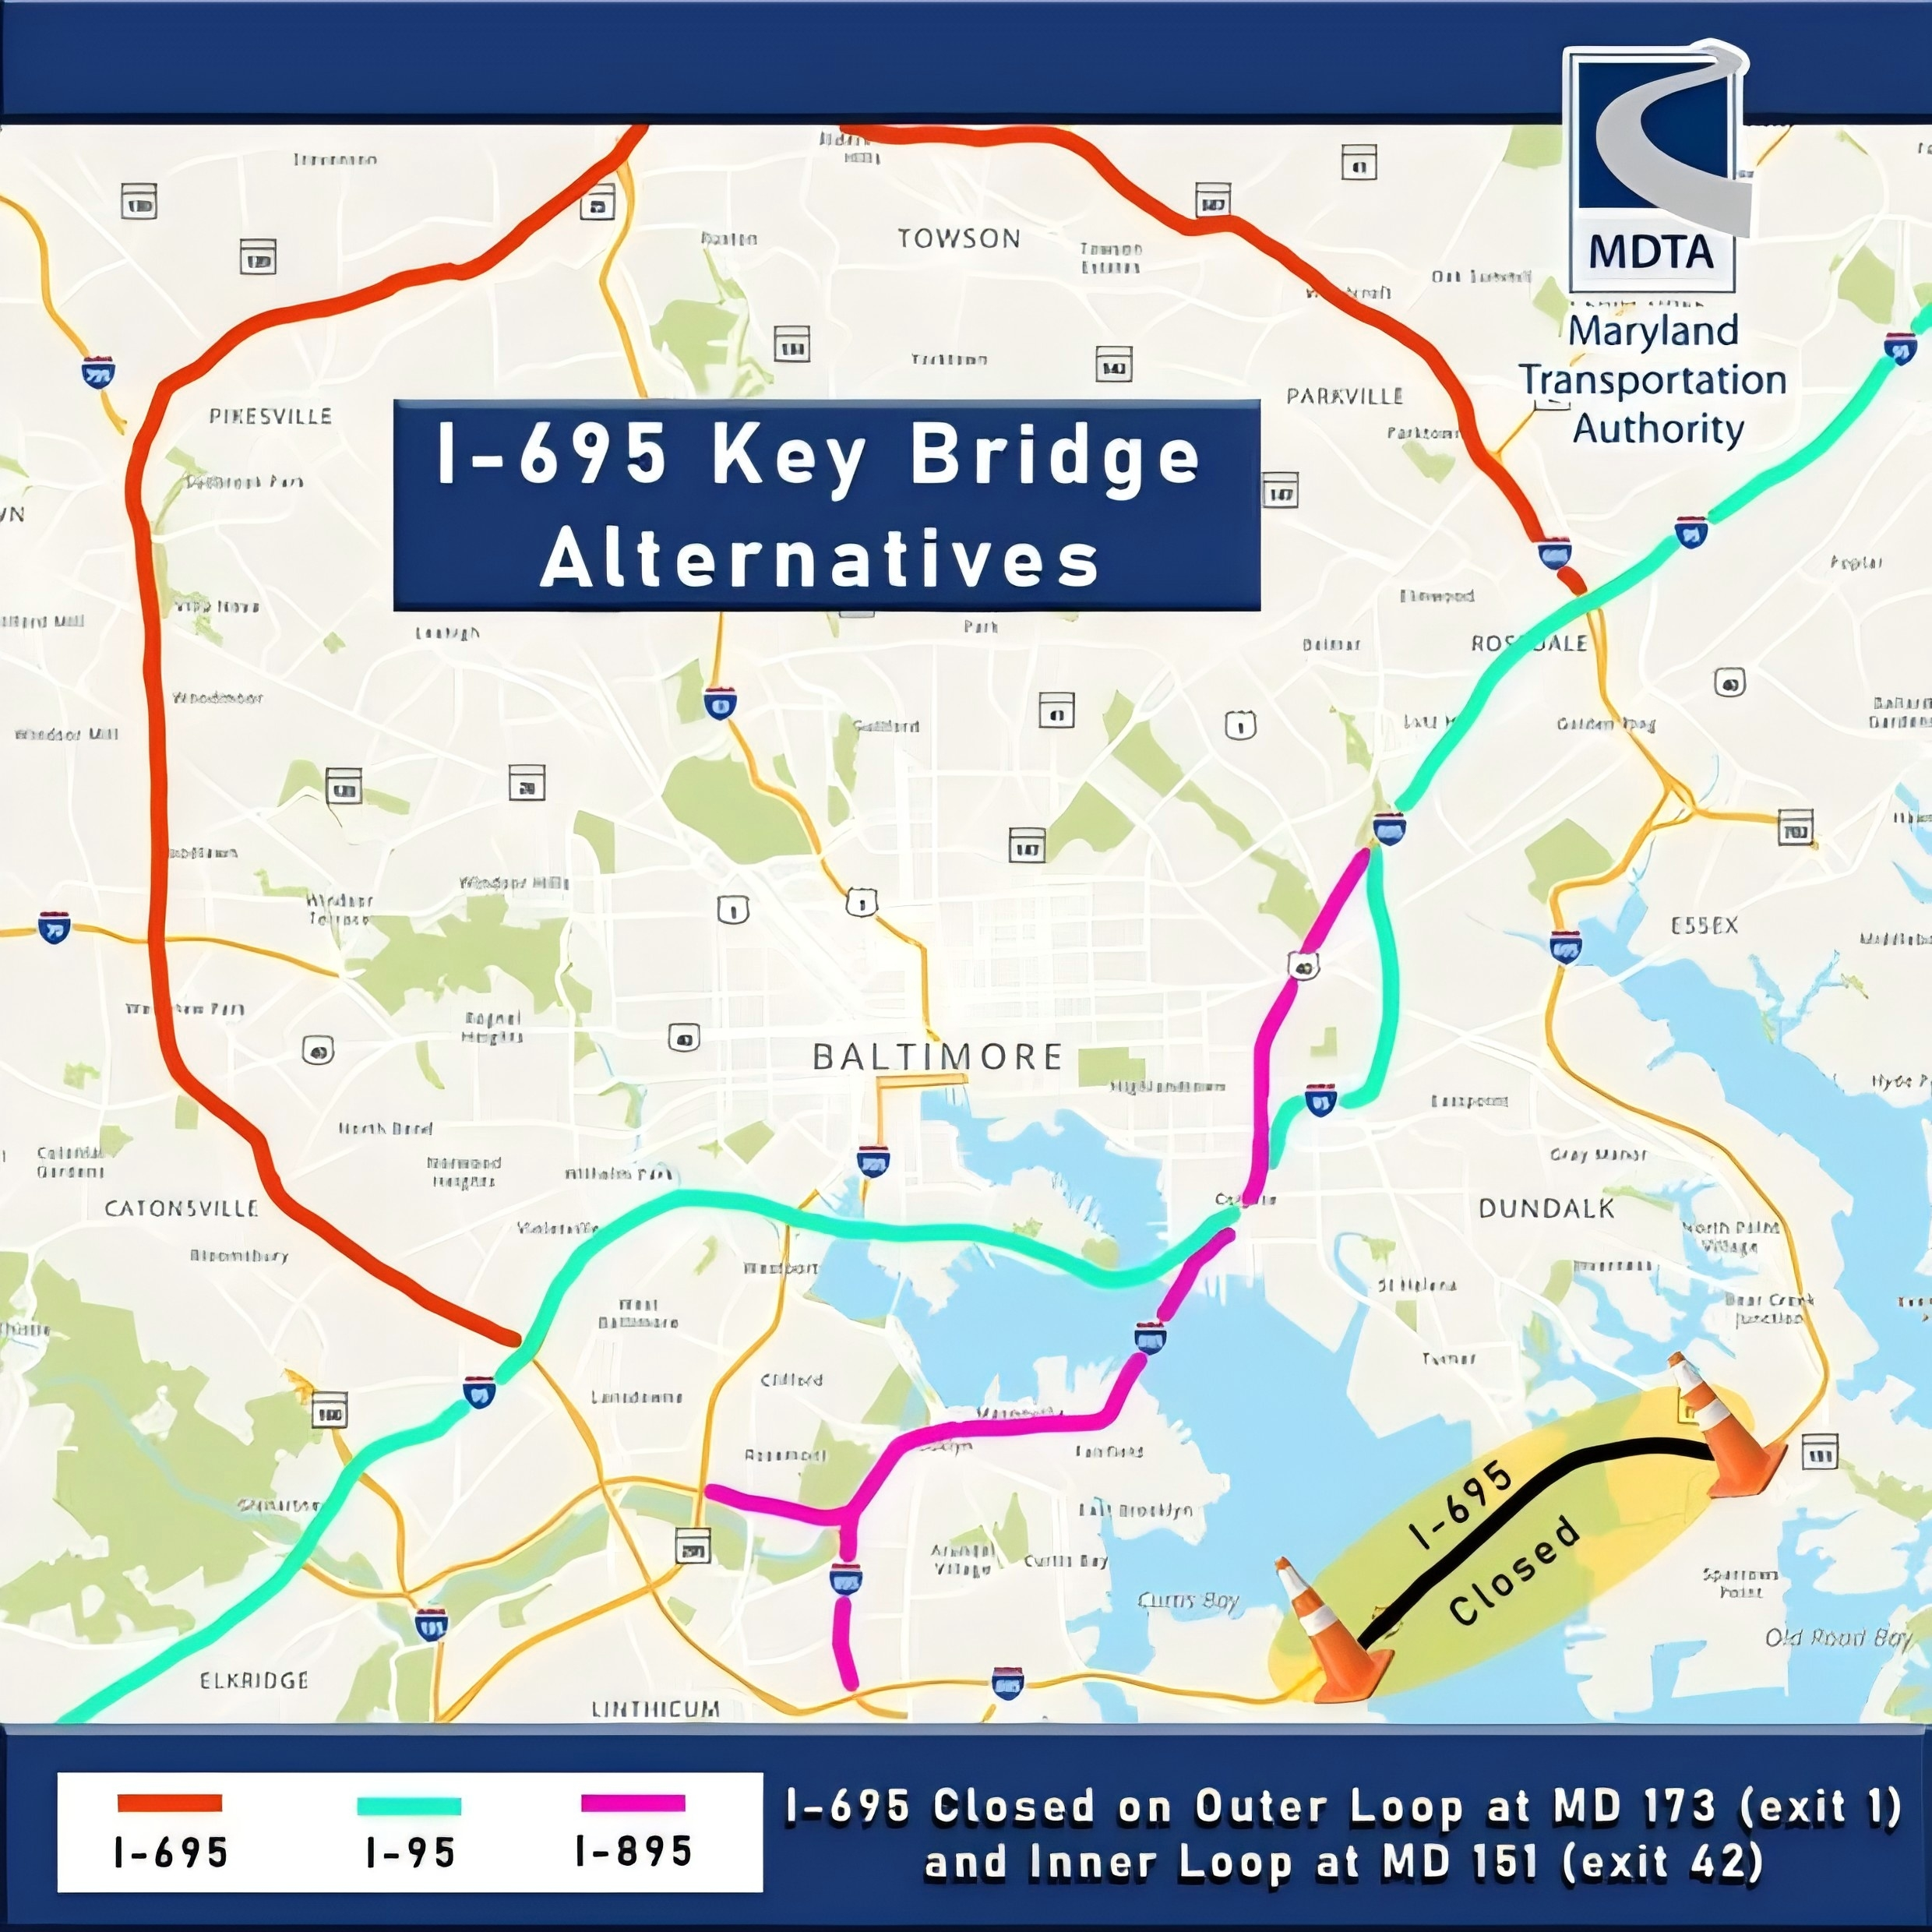
\includegraphics[width=0.55\linewidth]{figures/gk-pyc8xsaejjhz-1.jpg}
    \caption{Traffic Impacts and Detour Routes After Francis Scott Key Bridge Collapse in Baltimore}
    \label{fig:enter-label}
\end{figure}

It is clear that for businesses in the port area—those with heavy cargo transportation needs that once relied on the bridge—the impact has been considerable. Forced to take detours, the traffic burden has now been redirected largely to I-95 and I-895.

\begin{figure}[htbp]
    \centering
    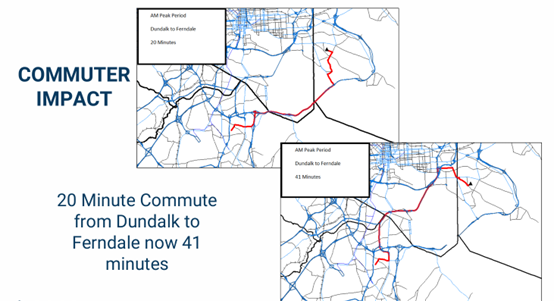
\includegraphics[width=0.75\linewidth]{figures/b801065ea2bf67a07928719f7908005.png}
    \caption{FRANCIS SCOTT KEY BRIDGE IMPACT ANALYSIS，2024，06}
    \label{fig:enter-label}
\end{figure}


In the port area, where heavy cargo transportation demands prevail, business owners who once depended on the bridge have been notably affected. Forced to detour, the traffic burden has shifted dramatically to I-95 and I-895. The traffic impact analysis report reveals that, from the standpoint of time costs, the detour has nearly doubled travel time—rising from the previous 20 minutes to 41 minutes—thus substantially intensifying congestion.

\begin{figure}[htbp]
    \centering
    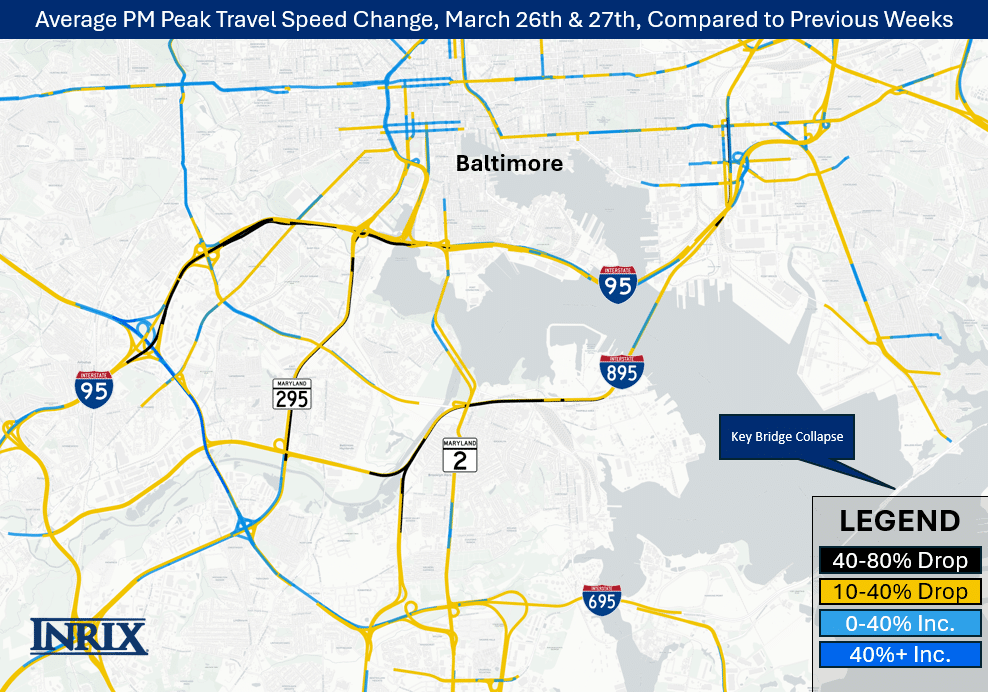
\includegraphics[width=0.6\linewidth]{figures/f63b86a27be347b8dfa4e9440ec383f.png}
    \caption{Initial Traffic Impacts Following the Collapse of the Key Bridge - INRIX}
    \label{fig:enter-label}
\end{figure}

Analysis of traffic data from Maryland reveals that the early impacts following the Dundalk Bridge collapse were substantial. On Tuesday and Wednesday after the incident, speeds along I-95, I-895, and MD-295 significantly slowed. On the Harbor Tunnel Thruway (I-895), speeds dropped to as low as 10 mph on certain segments, while near the I-695 interchange on I-95, speeds fell to 14 mph. Additionally, traffic speeds between the I-895 and I-95 interchanges reached a low of 13 mph.

According to data from MDOT\_SHA\_Annual\_Average\_Daily\_Traffic\_Baltimore.csv, the Key Bridge typically sees an average of 40,000 vehicles daily. Prior to the collapse, 72\% of these were passenger vehicles, 20\% were local fleets and delivery trucks, and 8\% were semi-trucks. The collapse has not only impacted daily commuters but also caused significant disruptions for businesses reliant on the bridge for cargo transport.

\subsection{Analysis from the Perspective of Different Stakeholders}

Following the collapse of the bridge, certain roads were damaged and are no longer accessible. By cross-referencing the table detailing the preferred locations and preferences of various stakeholders, we can determine the key travel destinations. An analysis of traffic conditions is then conducted, considering the travel preferences of these stakeholders.

\textbf{For Urban Residents:}

\begin{figure}[htbp]
    \centering
    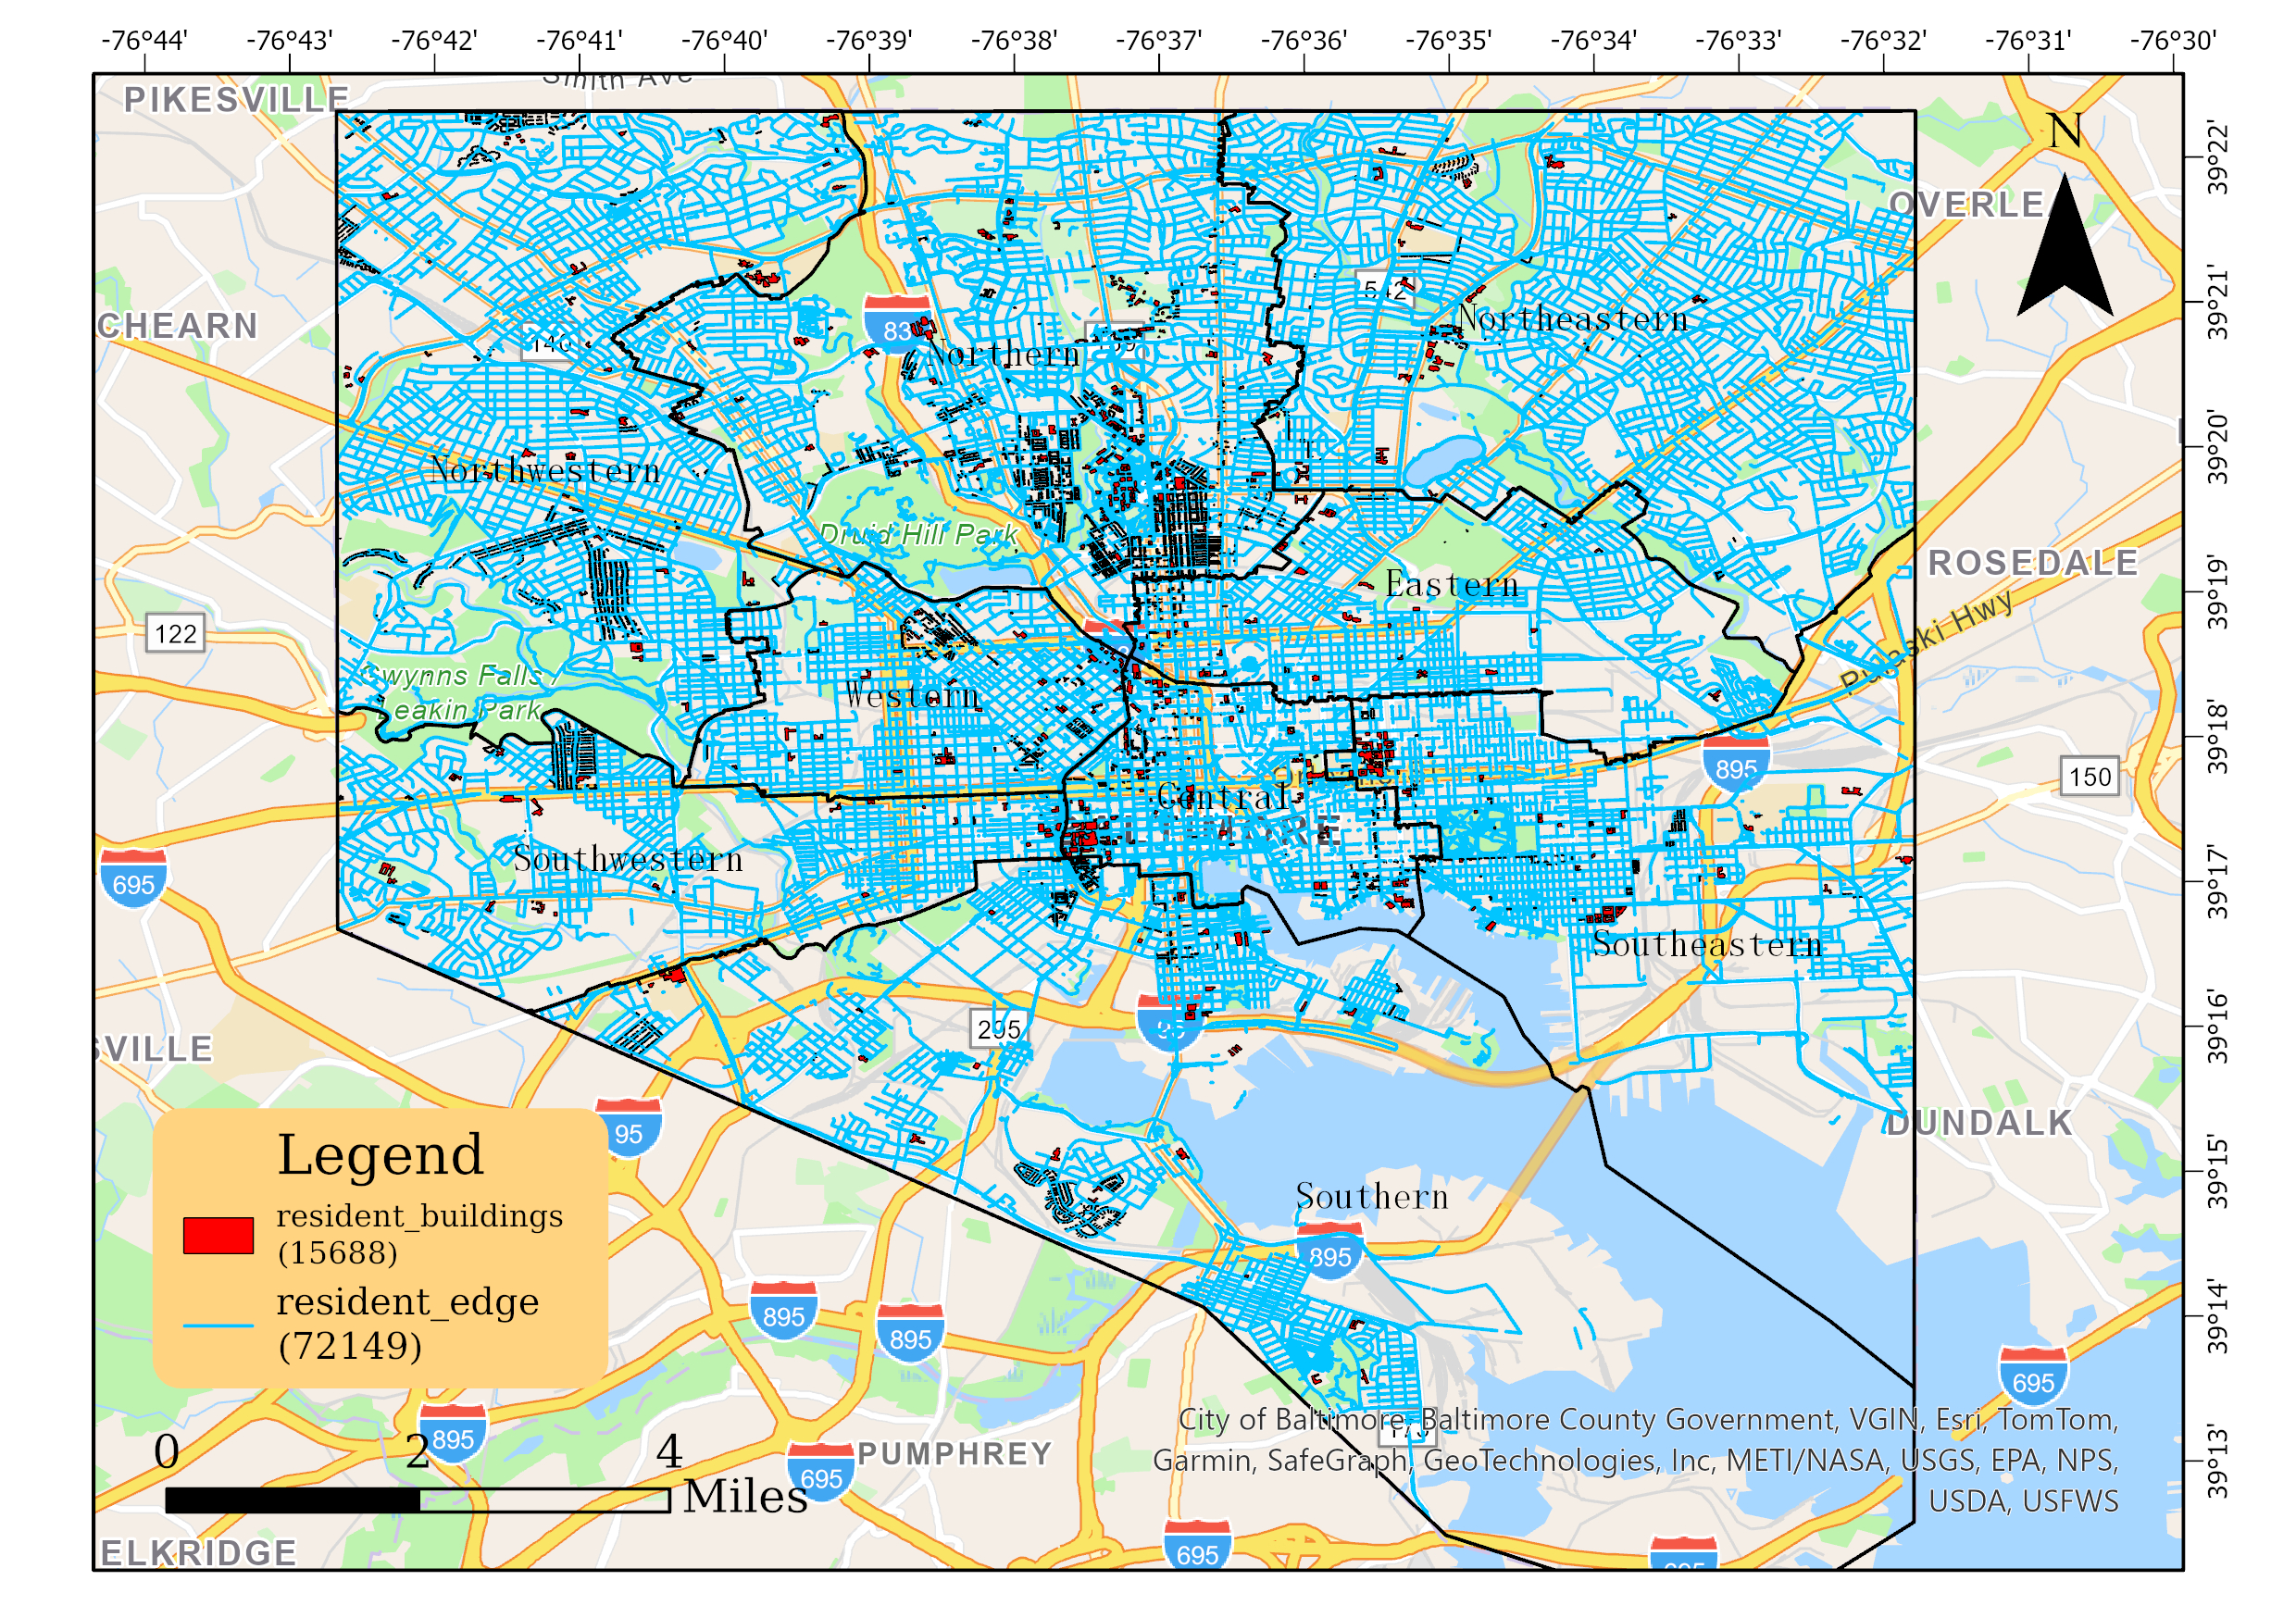
\includegraphics[width=0.6\linewidth]{figures/resident_all.jpg}
    \caption{Travel Location Preferences of Urban Residents}
    \label{fig:enter-label}
\end{figure}

The travel preferences of urban residents are largely centered around convenience in daily life and the ease of commuting. After the collapse of the bridge, those who had depended on it for their daily commutes are now forced to explore alternative routes, resulting in an increase in both commuting time and costs. This not only lengthens commute times but may also negatively impact their overall quality of life.

\textbf{For Business Owners:}

\begin{figure}[htbp]
    \centering
    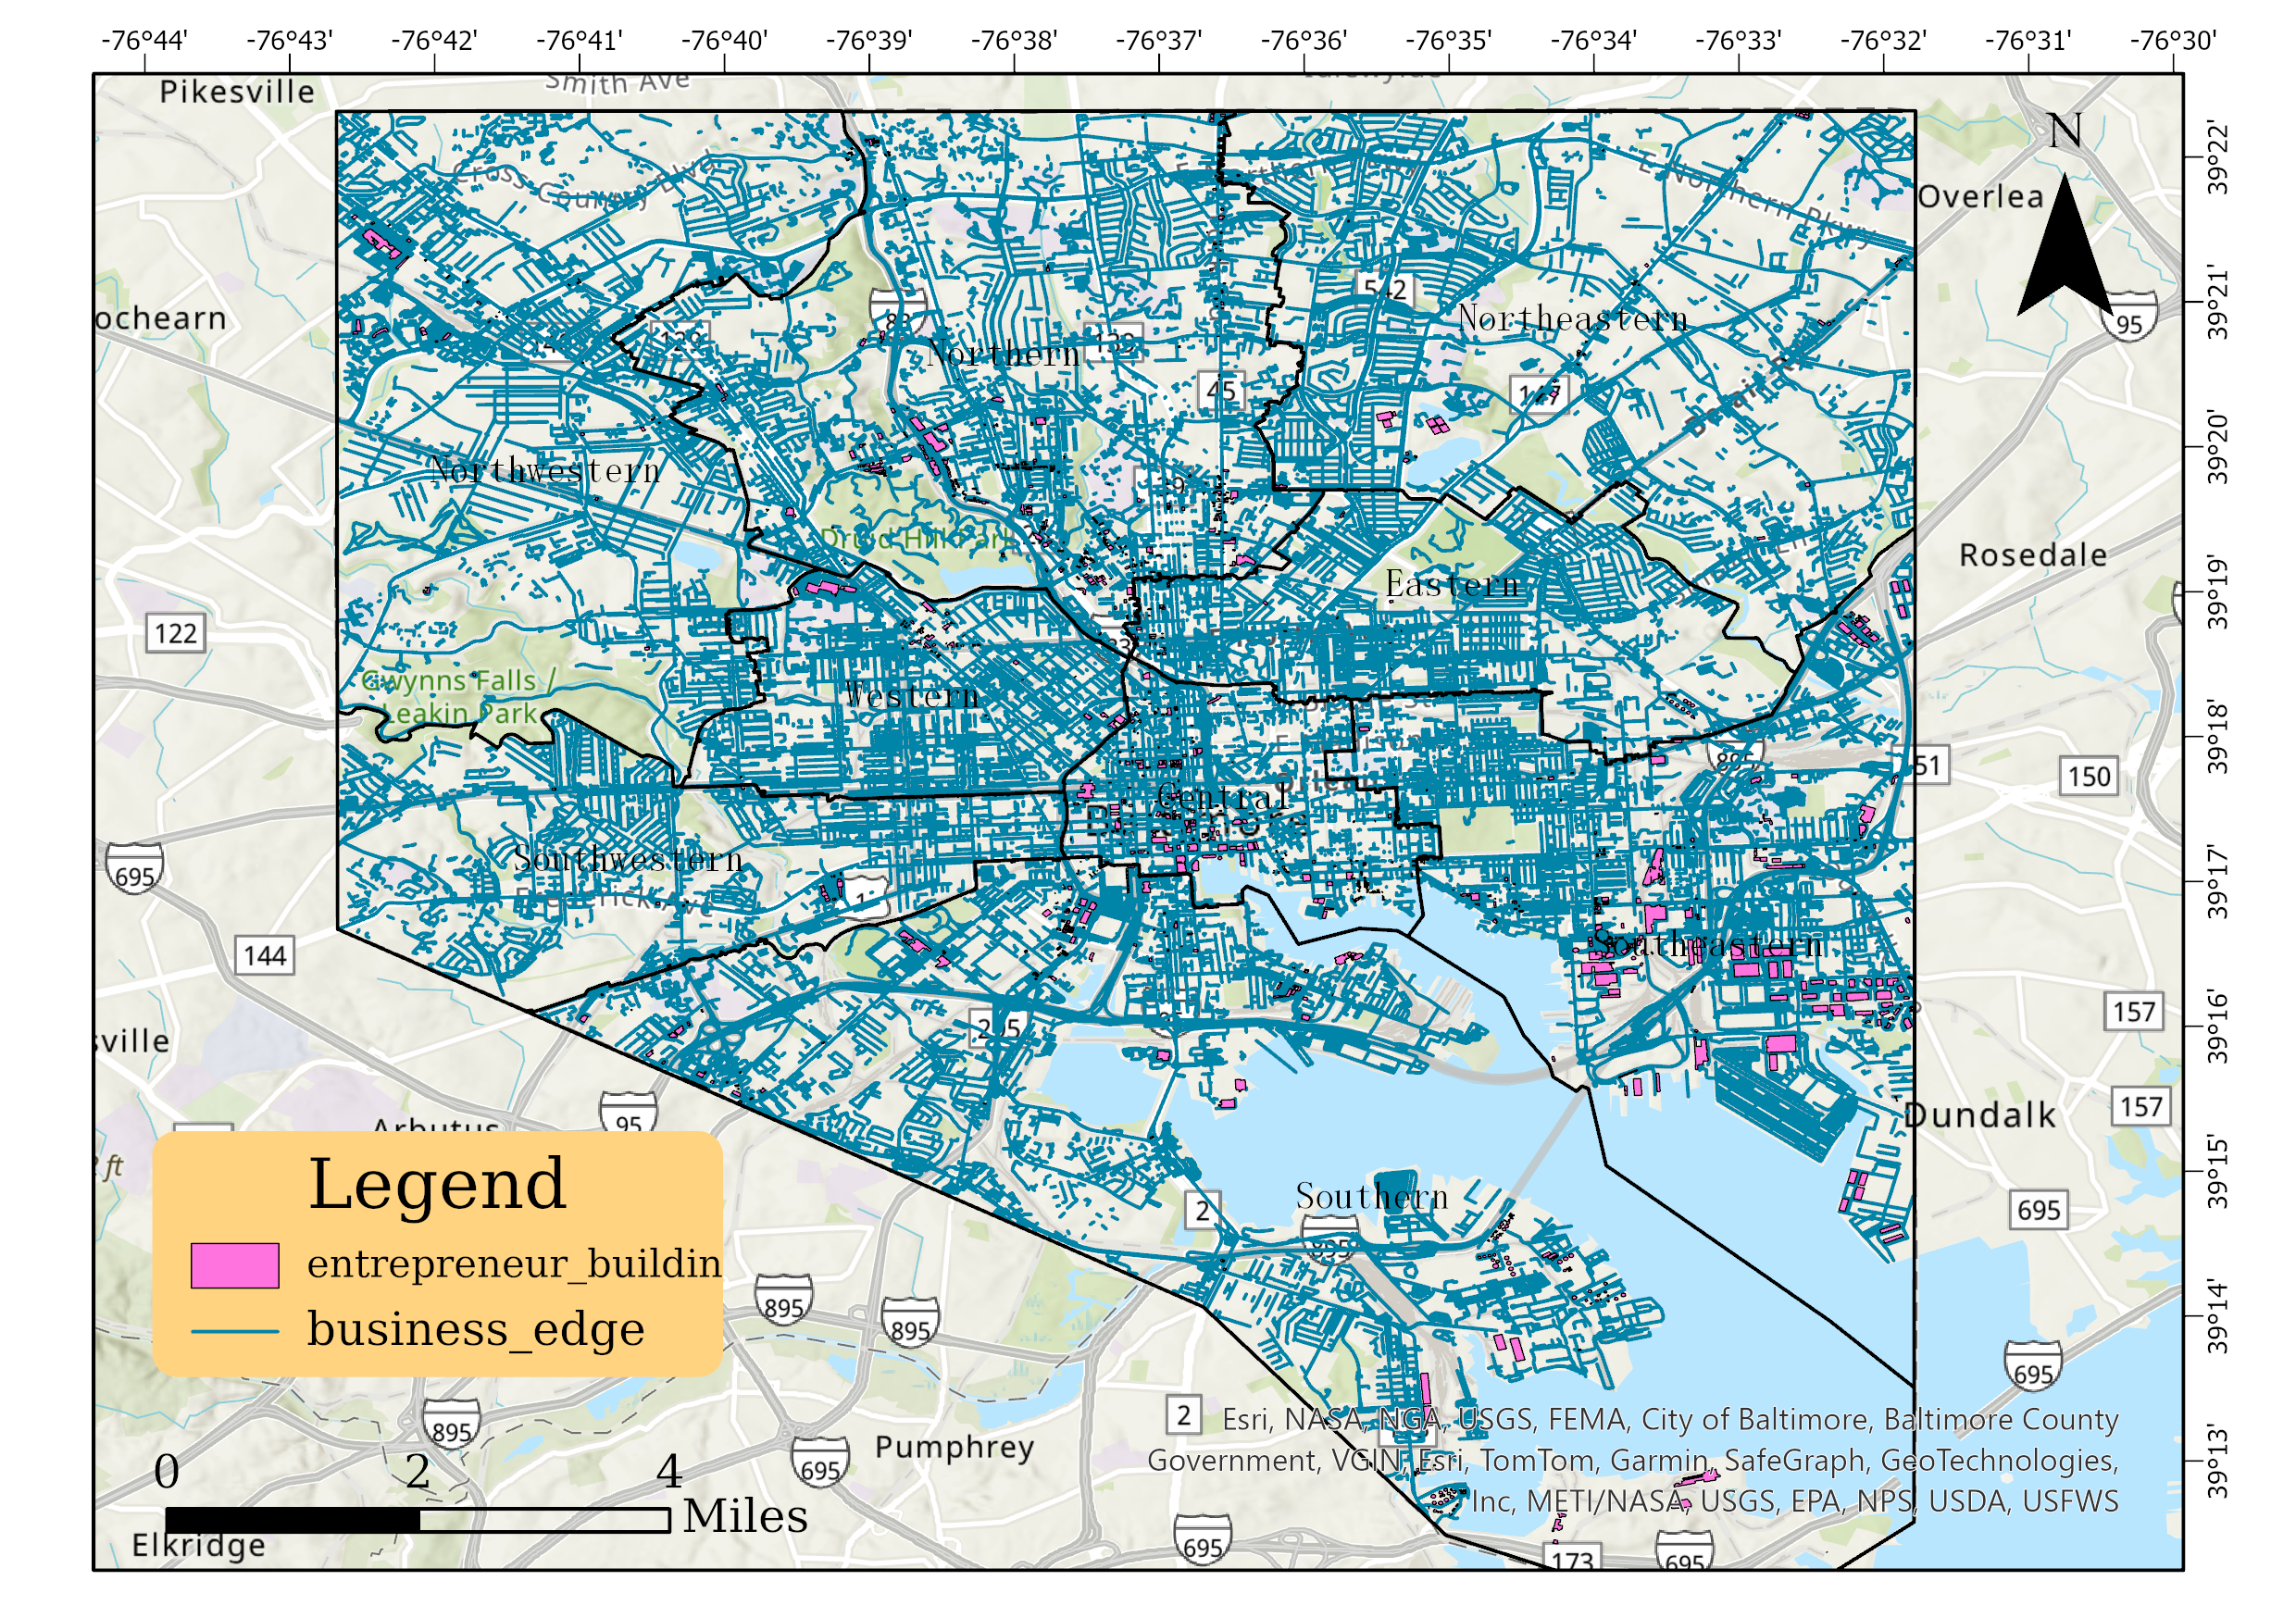
\includegraphics[width=0.6\linewidth]{figures/abf6c4dbbe3329da6fb206abdb37e55.jpg}
    \caption{Travel Location Preferences of Entrepreneurs}
    \label{fig:enter-label}
\end{figure}

Entrepreneurs prioritize the efficiency of cargo transportation and accessibility to commercial areas. The collapse of the bridge has had a profound impact on their business operations, especially for those dependent on the bridge for the movement of goods. As a result, entrepreneurs must rely on both primary and secondary roads for logistics, leading to potential supply chain disruptions, increased costs, and longer delivery times, all of which undermine operational efficiency. Service roads are also crucial for businesses, particularly those that frequently handle goods. The bridge collapse has caused an uptick in traffic on these roads, further impeding the logistical efficiency of these enterprises.

\textbf{For Tourists:}

\begin{figure}[htbp]
    \centering
    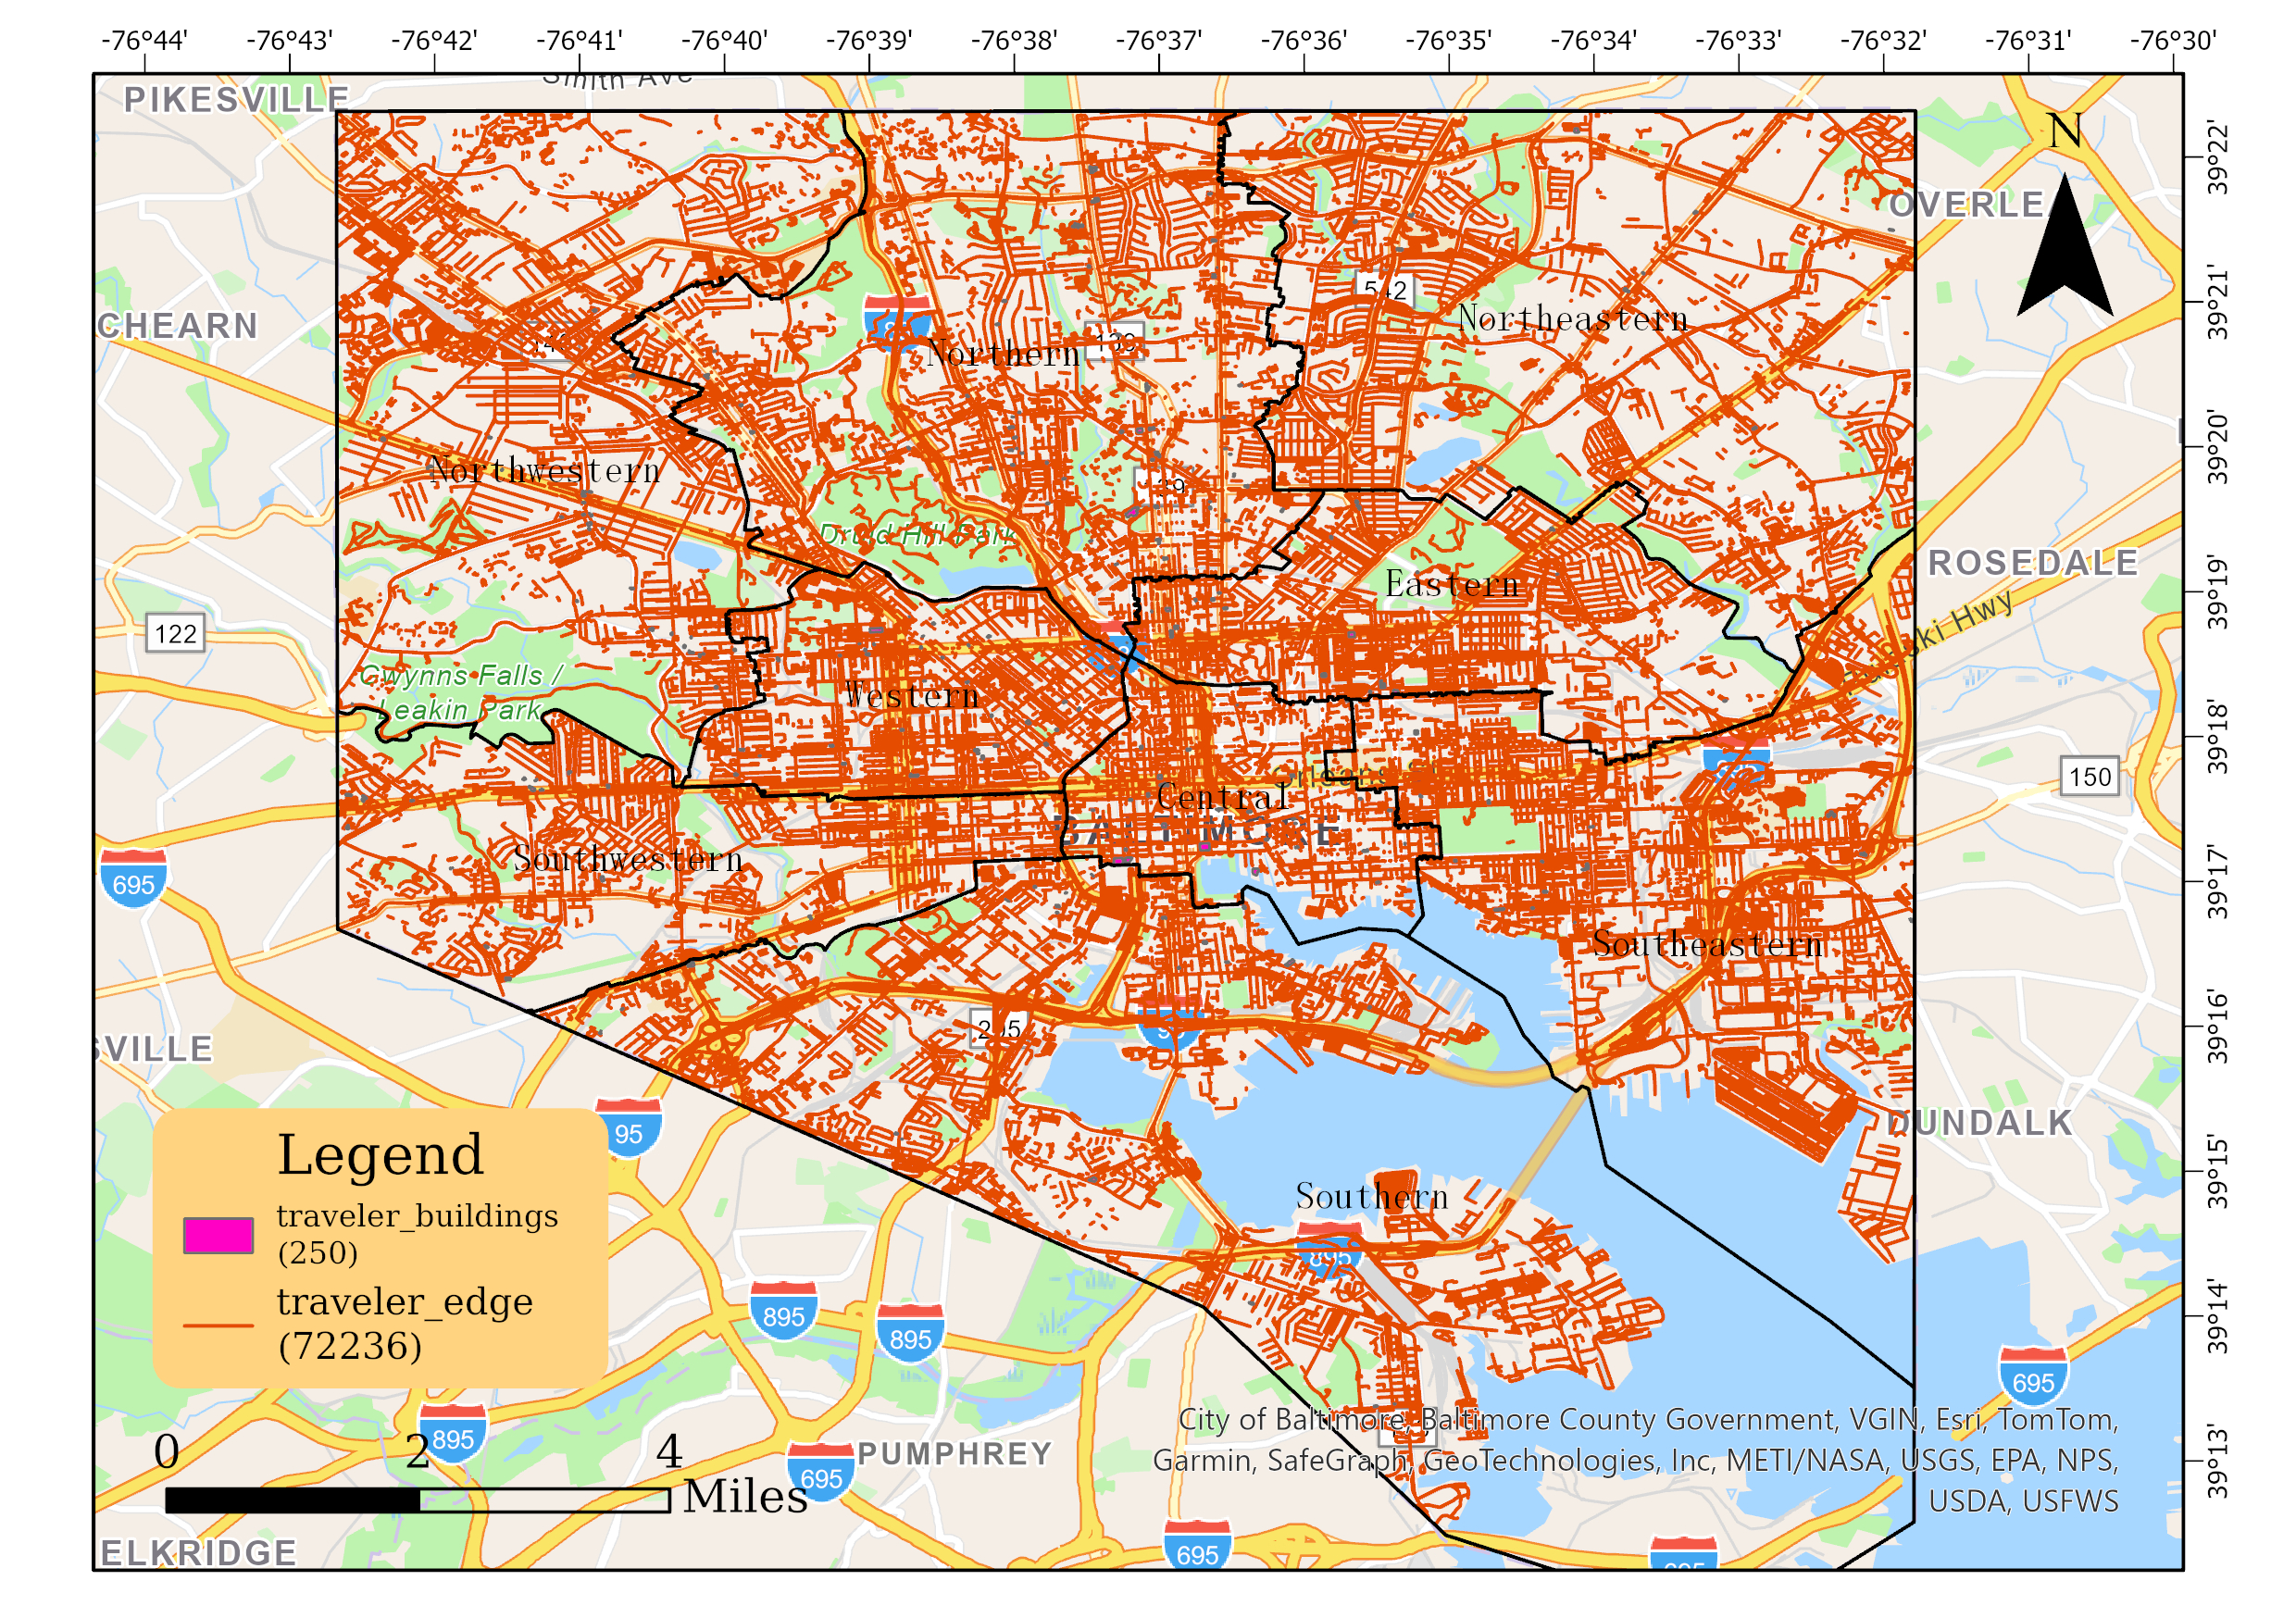
\includegraphics[width=0.6\linewidth]{figures/traveler_all.jpg}
    \caption{Travel Location Preferences of Tourists}
    \label{fig:enter-label}
\end{figure}


Tourists prioritize easy access to major attractions. The collapse of the bridge may compel them to change their travel plans, potentially diminishing their overall experience. With the reduced accessibility of certain attractions, tourists might be forced to find alternative routes, lowering the chances of visiting certain sites. Moreover, tourists often rely on walking, cycling, and public transportation to explore the city, and the collapse of the bridge could disrupt the availability and convenience of these modes, affecting their travel experience.


\section{Optimization and Development of the Transportation Infrastructure}

In light of the particular concerns of urban residents regarding travel, especially free modes of transportation such as walking and cycling paths, it is essential to assess the current state of the transportation system to determine if it meets the daily needs of residents. Below are the detailed analysis steps and key considerations:

\subsection{Analysis of the Current Road Conditions}

\begin{figure}[htbp]
    \centering
    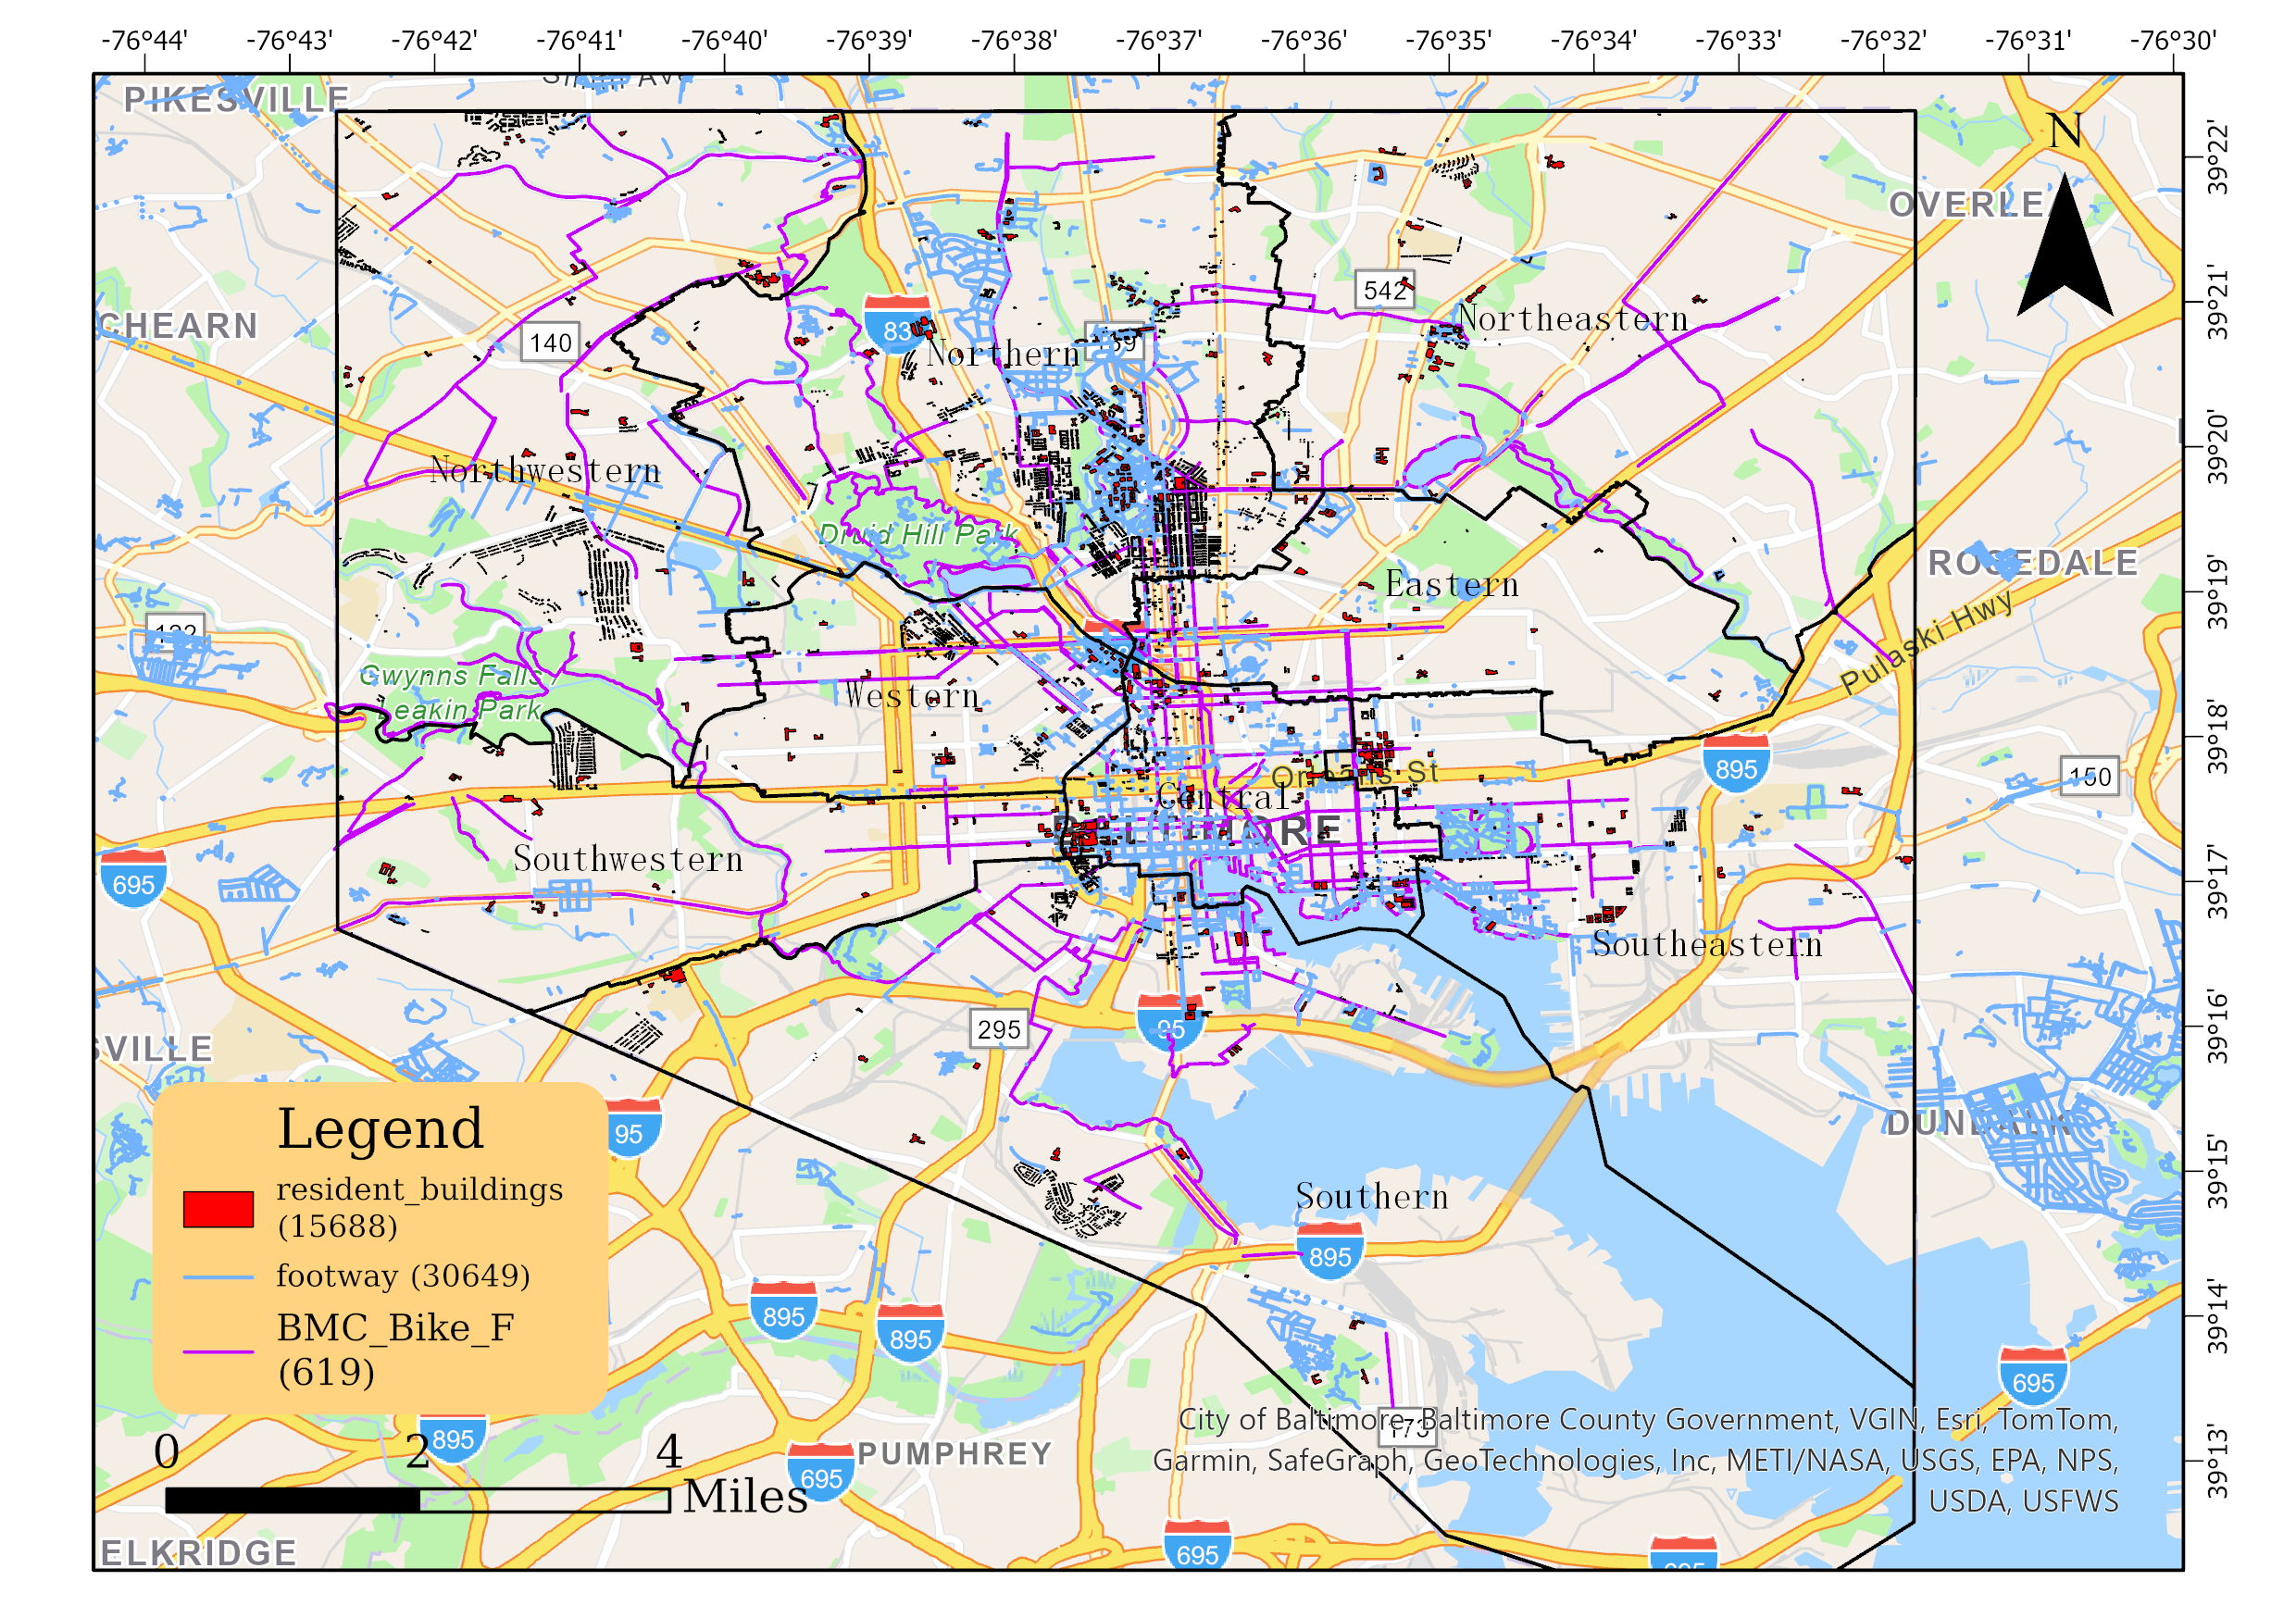
\includegraphics[width=0.75\linewidth]{figures/footway1.jpg}
    \caption{Existing Transportation Network}
    \label{fig:enter-label}
\end{figure}

Observe and analyze the current transportation network to assess its efficiency and coverage. Utilizing network models allows for the identification of areas with sparse infrastructure, where pedestrian and cycling paths may be insufficient or entirely lacking. These areas may not meet the travel demands of residents, potentially leading to mobility challenges. By examining the existing network’s capacity to support sustainable modes of transport, we can highlight gaps in infrastructure and recommend necessary improvements to ensure accessibility and convenience for all users.

\subsection{Road Planning}

The application of Geospatial Technologies (GST), including Remote Sensing (RS) and Geographic Information Systems (GIS), can significantly enhance the planning and implementation of public transportation infrastructure in Baltimore. These technologies offer powerful tools for the collection, processing, and analysis of spatial data, enabling more scientifically grounded and precise road planning\cite{litman2009}. By leveraging these advanced technologies, urban planners can optimize transportation networks, improve decision-making processes, and better align infrastructure development with the evolving needs of the city’s residents and visitors.

\begin{itemize}
    \item \textbf{Data Collection and Processing}
            \begin{itemize}
                \item \textbf{GIS Data:} ArcGIS software is employed to process and analyze GIS datasets, including land use/land cover, roads, soil, elevation, and demographic data. These datasets are instrumental in assessing the suitability of locations for bike lanes and pedestrian pathways.
            \end{itemize}
            


    \item \textbf{Land Use/Land Cover (LULC) Analysis}
    
            \begin{itemize}
                \item \textbf{LULC Classification:} Remote sensing technology is used to classify the Perring Parkway corridor’s LULC, identifying various types of geospatial features. The classification results indicate that built-up areas cover 31\%, vegetation accounts for 56\%, and water bodies/wetlands make up 13\%. This information aids in pinpointing optimal locations for bike lanes and walking paths.

                \item \textbf{NDVI Analysis:} The Normalized Difference Vegetation Index (NDVI) is calculated to assess vegetation coverage. Areas with lower NDVI values typically have sparse vegetation, making them more suitable for development, including the construction of biking and walking infrastructure.
            \end{itemize}


    \item \textbf{GIS Analysis}
    
            \begin{itemize}
                \item \textbf{Buffer Analysis:} A buffer zone is generated around the Perring Parkway corridor to identify potential locations for the bike lane. The buffer width includes both the existing road width and the planned width for the bike lane.

                \item \textbf{Clipping and Overlaying:} Using GIS’s clipping and overlay functions, land use types and soil types within the buffer zone are analyzed. This information is crucial for evaluating the feasibility and suitability of the proposed bike lane.

                \item \textbf{Attribute Table Generation:} An attribute table is generated, containing detailed data on road width, lane width, median width, and sidewalk width. This table provides essential information for the design of the bike lane, ensuring that all relevant physical parameters are considered in the planning process.
            \end{itemize}


    \item \textbf{Site Selection for Roadway}

            \begin{itemize}
                \item \textbf{Optimal Location Selection:} Based on the results of the LULC classification and NDVI analysis, areas with sparse vegetation and suitable land use are selected as the most appropriate locations for the bike lanes. These areas are chosen to minimize environmental impact while ensuring accessibility and integration with the existing infrastructure.
            \end{itemize}
            
\end{itemize}

\newpage
\subsection{Recommended Road Construction Plan}

\begin{figure}[htbp]
    \centering
    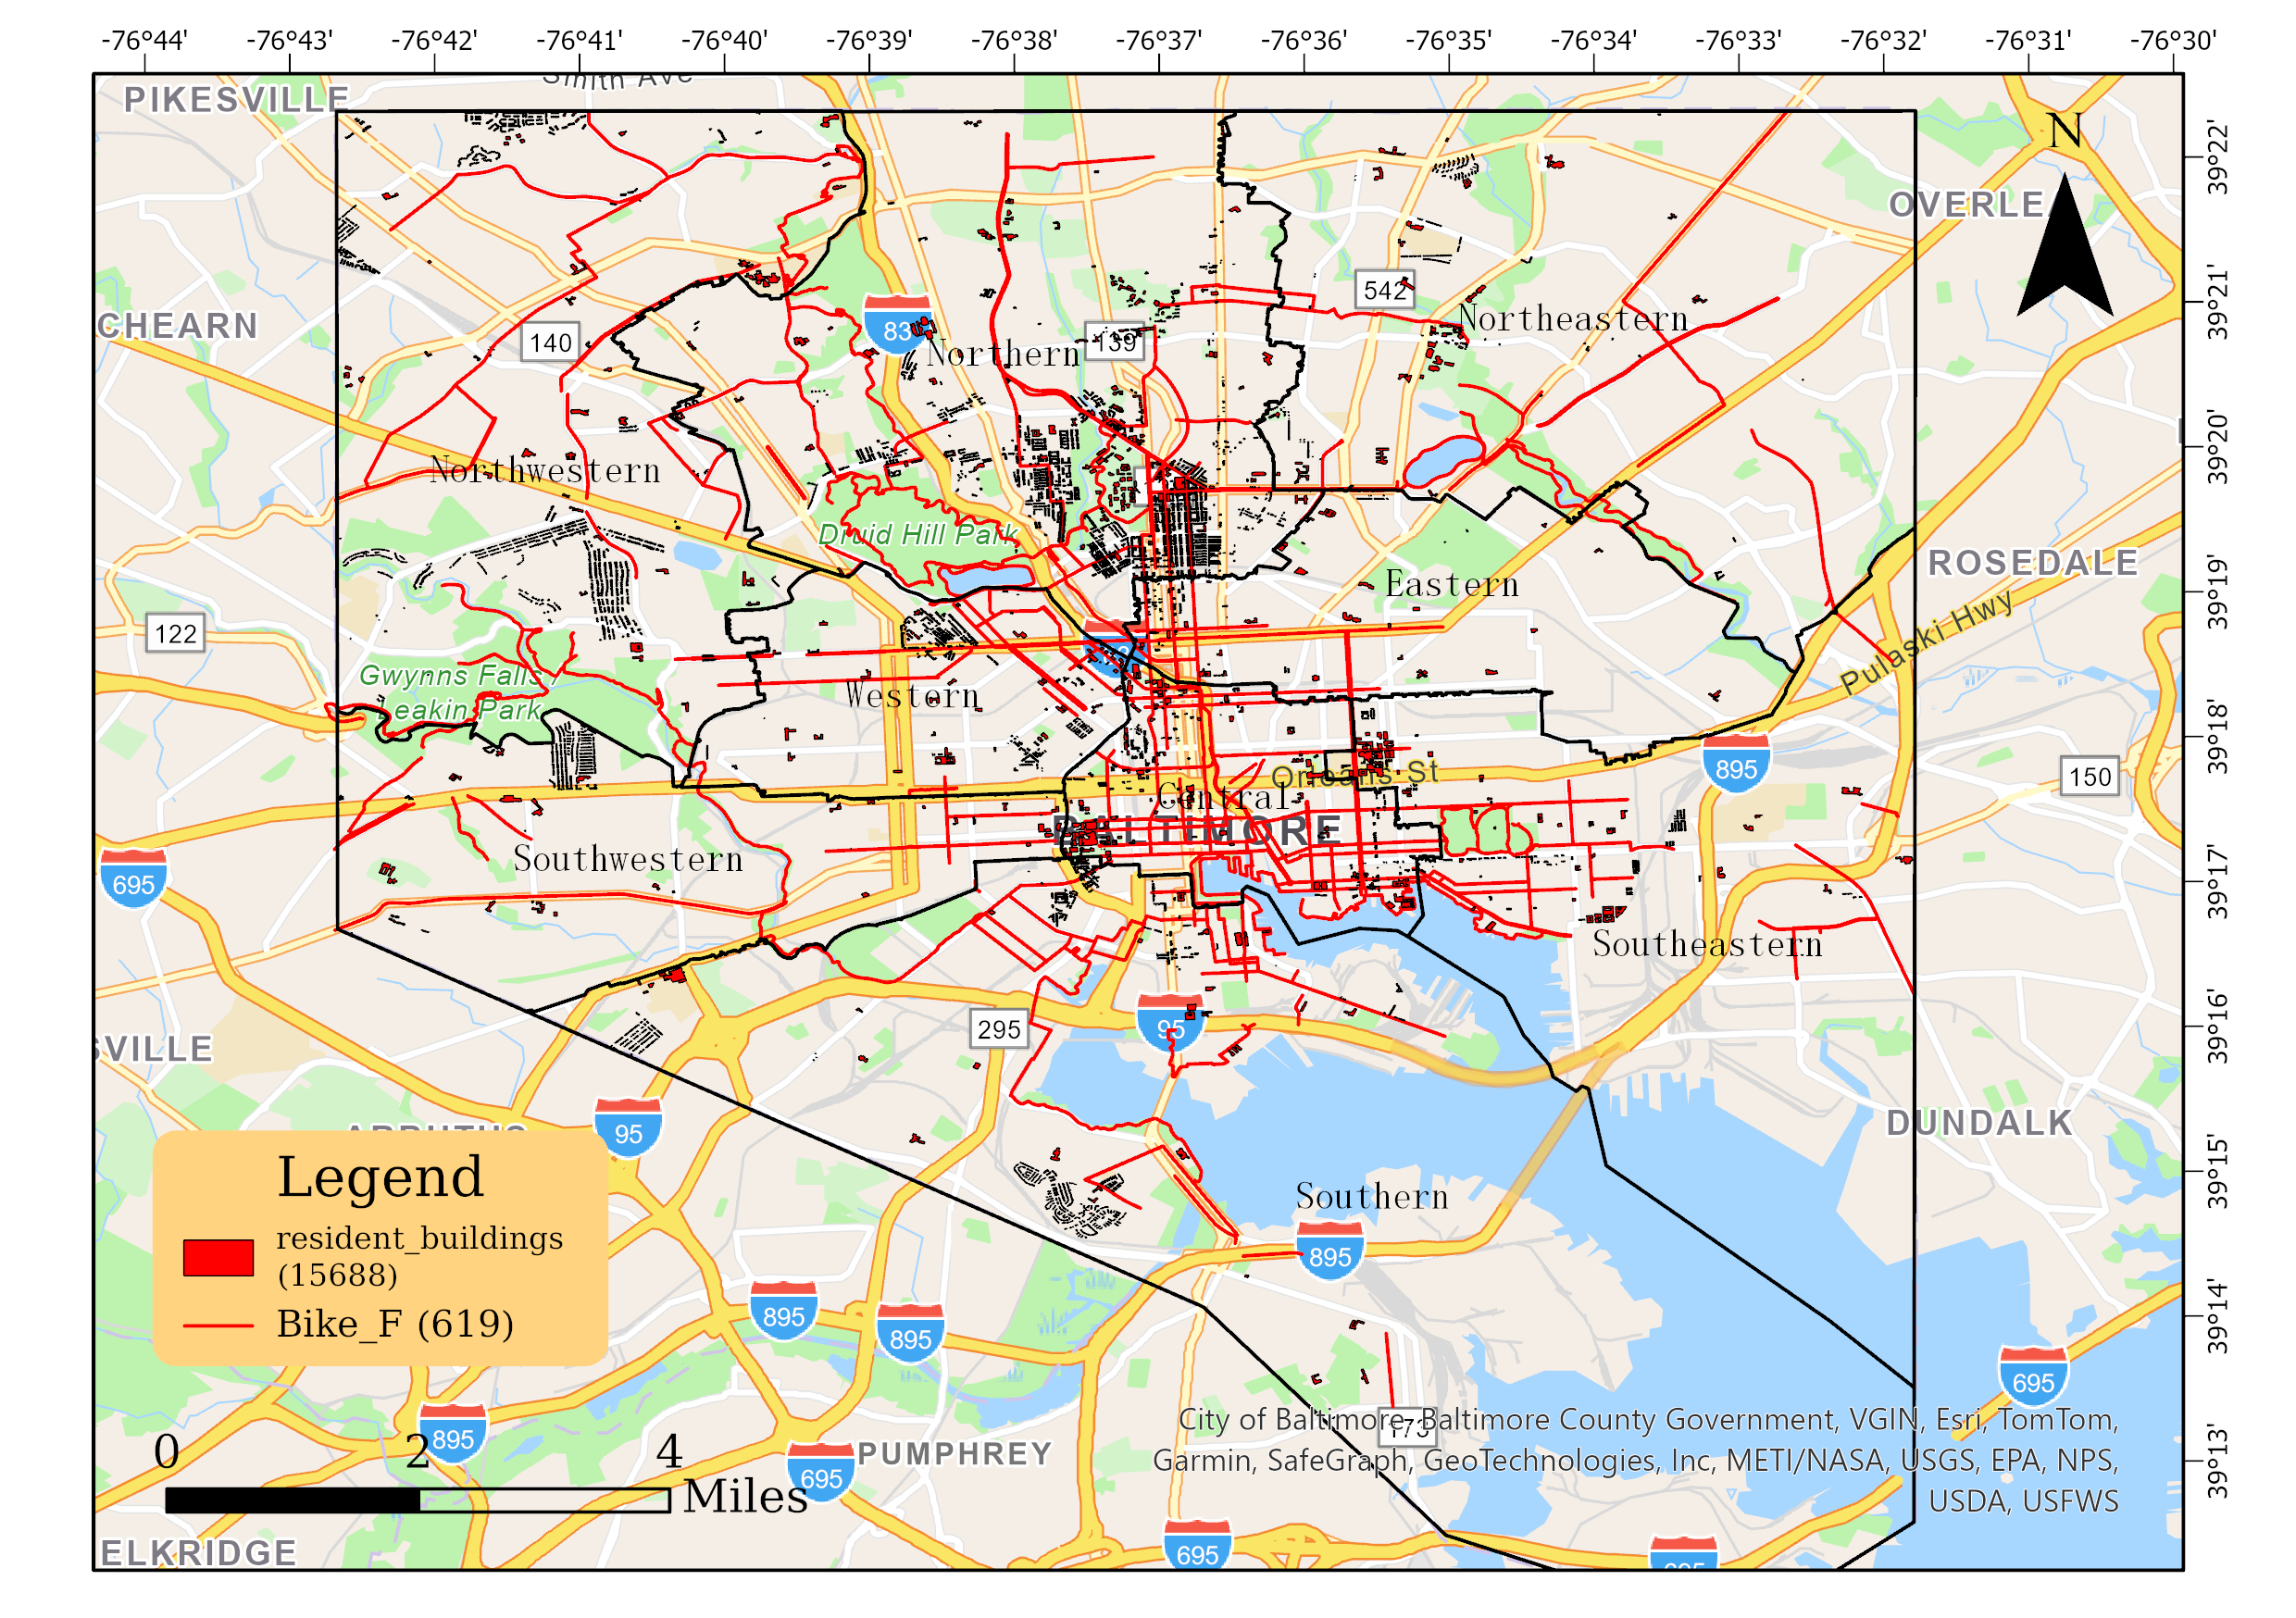
\includegraphics[width=0.75\linewidth]{figures/Bike.jpg}
    \caption{Road construction plan recommendation}
    \label{fig:enter-label}
\end{figure}

The optimal locations for the construction of new bike lanes should be selected to connect with the existing bike lane network, thereby enhancing connectivity and extending the coverage of the network. In areas with high foot traffic, improvements or new pedestrian paths should be introduced to provide a safer and more comfortable walking environment.

This plan\cite{afro2025} will not only strengthen Baltimore's public transportation infrastructure but also improve residents' travel convenience and overall quality of life. Moreover, it will promote healthier and more environmentally-friendly modes of transportation, contributing to the city’s sustainable urban development goals.



\section{Conclusion}

This study\cite{mta2025} takes the collapse of the Francis Scott Key Bridge in Baltimore as a case study to systematically explore the impact of bridge failure on urban transportation networks and to propose strategies for network reconstruction and optimization. By employing the Voronoi diagram method for traffic zone partitioning and constructing a road network model based on topological structures, coupled with traffic flow data (e.g., AADT, AAWDT) and preference indicators derived , this research evaluates regional traffic accessibility. Moreover, it offers optimization recommendations tailored to the needs of various stakeholders, including city residents, entrepreneurs, and tourists.

First and foremost, bridges serve as pivotal nodes within urban transportation networks, and their collapse can exert profound effects on traffic flow and economic activity. The failure of the Francis Scott Key Bridge not only obstructed daily commutes but also inflicted considerable disruption on freight transportation, tourism, and regional economic development. The findings of this study highlight that, in the wake of the collapse, traffic congestion significantly shifted to other major highways (such as I-95 and I-895), leading to increased commute times and transportation costs.

Additionally, this study utilizes Voronoi partitioning to define traffic zones and leverages ArcGIS for spatial analysis and visualization, quantifying new traffic accessibility indicators, such as the average traffic zone area, the density of traffic zones per square kilometer, and the accessibility index. These metrics provide a scientific basis for identifying the vulnerabilities within the transportation network. Furthermore, the topologically-based traffic flow model allows for an analysis of node and edge connectivity, with the integration of traffic flow data refining network weights, thereby supporting more precise transportation planning.

Tailored models for different stakeholders have been developed to quantify their preferences regarding transportation networks. The study reveals that city residents prioritize daily convenience, preferring walking, cycling, and public transport; entrepreneurs, concerned with logistics efficiency, emphasize the accessibility of commercial and industrial districts; while tourists value convenient access to tourist attractions and hotels. The collapse of the bridge has had varying impacts on the travel needs of these groups: increased commute times for residents, higher transportation costs for entrepreneurs, and a diminished travel experience for tourists.

Based on these findings, this study proposes specific recommendations for optimizing the transportation system. For city residents, the study suggests the construction of pedestrian pathways and cycling lanes, the improvement of the existing road network, and the enhancement of public transportation connections to increase overall accessibility. For entrepreneurs, it recommends optimizing the layout of both major and minor roads to alleviate transportation pressures and ensure the smooth operation of supply chains. For tourists, the study advocates for the enhancement of transportation facilities around tourist areas to improve their experience and foster tourism development. Additionally, the introduction of Intelligent Transportation Systems (ITS) is recommended to monitor traffic flow in real time, optimize signal control, and improve route planning, thereby enhancing traffic efficiency.

In conclusion, this research provides a solid scientific foundation for urban transportation planning and holds significant practical value. The findings suggest that increasing road redundancy, promoting green transportation options (such as walking, cycling, and public transit), and fostering multi-stakeholder collaboration can substantially improve the resilience, efficiency, and equity of transportation systems, offering more convenient and sustainable transportation services for residents, businesses, and tourists. Future studies should explore the integration of intelligent traffic management and green transportation solutions to promote the sustainable development of urban transportation systems and provide guidance for responding to unforeseen infrastructural failures.










\newpage
\begin{thebibliography}{9}

\bibitem{boeing2024}
Boeing, G. 2024. ``Modeling and Analyzing Urban Networks and Amenities with OSMnx.'' Working paper. \textit{URL:} \url{https://geoffboeing.com/publications/osmnx-paper/OpenStreetMap}.

\bibitem{openstreetmap2025}
OpenStreetMap contributors. \textit{OpenStreetMap} [Internet]. [place of publication unknown]: OpenStreetMap Foundation; 2025 [cited 2025 Jan 10]. Available from: \url{https://www.openstreetmap.org}.

\bibitem{mdot2025}
Maryland Department of Transportation. \textit{MDOT SHA Annual Average Daily Traffic (AADT) Locations} [Internet]. Baltimore, MD: Maryland Department of Transportation; 2025 [cited 2025 Jan 10]. Available from: \url{https://data.imap.maryland.gov/datasets/maryland::mdot-sha-annual-average-daily-traffic-aadt-locations/explore}.

\bibitem{litman2009}
Litman, T. A. (2009). \textit{Sustainable Transportation Indicators: A Recommended Research Program for Developing Sustainable Transportation Indicators and Data}.

\bibitem{afro2025}
New initiative aims to heal divide caused by West Baltimore’s infamous ‘Highway to Nowhere’. \textit{Afro}. 2025 Jan 1. Available from: \url{https://afro.com/new-initiative-aims-to-heal-divide-caused-by-west-baltimores-infamous- \\ highway-to-nowhere/}.

\bibitem{mta2025}
Maryland Transit Administration. \textit{MTA Performance}. SCIRP. Available from: \url{https://www.scirp.org/reference/referencespapers?referenceid=3900167}.

\bibitem{edelsbrunner1985voronoi}
Edelsbrunner, H., and Seidel, R. 1985. ``Voronoi diagrams and arrangements.'' In \textit{Proceedings of the First Annual Symposium on Computational Geometry}, 251--262.

\bibitem{farahani2013review}
Farahani, R. Z., Miandoabchi, E., Szeto, W. Y., and Rashidi, H. 2013. ``A review of urban transportation network design problems.'' \textit{European Journal of Operational Research}, 229(2), 281--302.

\bibitem{ji2012spatial}
Ji, Y., and Geroliminis, N. 2012. ``On the spatial partitioning of urban transportation networks.'' \textit{Transportation Research Part B: Methodological}, 46(10), 1639--1656.

\end{thebibliography}





\newpage

  \memodate{\today}
  \memoto{Mayor of Baltimore }
  \memofrom{Team \# \ 2503118}
  \memosubject{Post-Collapse Transportation System Optimization: Integrated Analysis of Benefits and Challenges}
  % \memologo{\LARGE I'm pretending to be a LOGO!}

  \begin{memo}[Memorandum]



This memorandum proposes two integrated infrastructure initiatives to enhance multimodal resilience, addressing equity and efficiency while mitigating the impacts of the recent bridge collapse. The initiatives leverage data-driven upgrades to non-motorized networks and arterial corridors, balancing immediate congestion relief with long-term sustainability.


\textbf{Project 1:Non-Motorized Infrastructure Expansion }

With a budget of \$73 million, this initiative focuses on enhancing pedestrian and bicycle networks along the Perring Parkway corridor. By constructing 5 km of protected bike lanes and upgrading pedestrian pathways in low-vegetation areas, the project is expected to reduce commute times by 15\% and cut transportation sector emissions by 10\% annually (12,800 tons of CO₂). Environmental benefits include a 37\% increase in green corridor coverage, improving heat resilience and disaster evacuation. The project faces a \$20.4 million funding gap and requires additional outreach funding of \$1.2 million to boost cycling adoption among the elderly, with only 43\% showing willingness according to AARP surveys.


\textbf{Project 2: Arterial Road Network Optimization}

To address congestion exacerbated by the bridge collapse on I-95 and I-895, a \$214 million optimization plan introduces three grade-separated port connectors and recalibrates 82 intersections. Simulations predict an 18\% reduction in freight logistics costs, a 25\% increase in I-95 throughput, and improved EMS response times from 12 to 8 minutes. Risks include a 34\% reduction in AM peak capacity during a 26-week realignment of Hanover Street, and a 5.1\% increase in traffic incidents during the driver adaptation phase. Ongoing maintenance will require \$12.6 million annually.


\textbf{Strategic Implementation Pathway }

To maximize synergies, we recommend prioritizing bicycle network expansion using existing CMAQ funds (\$48 million Phase 1 allocation) while initiating port corridor upgrades. An Interagency Task Force should oversee land acquisition, and real-time public dashboards should monitor construction impacts. Long-term success depends on legislative action to establish a transportation trust fund, ensuring maintenance budgets align with projected lifecycle costs.



\end{memo}







\end{document}


